\documentclass{article}
\usepackage{bbm}
\usepackage{graphicx}
\usepackage{placeins}
\usepackage[utf8]{inputenc}
\usepackage{amsmath}
\usepackage{listings}
\usepackage{booktabs}
\usepackage{rotating}


\usepackage[hidelinks]{hyperref}

\hypersetup{
    colorlinks=true,
    linkcolor=blue,
    filecolor=magenta,      
    urlcolor=blue,
}

\usepackage{float}      % For exact [H] placement of figures/tables
\usepackage{endnotes}   % For endnotes support
\usepackage{glossaries} % For glossary support
\usepackage{imakeidx}   % For index support
% ---------------------------------------
\usepackage{amsmath,amssymb,amsthm}
\usepackage{xcolor}
\numberwithin{equation}{section}

\theoremstyle{plain}
\newtheorem{property}{Property}[section]
\newtheorem{theorem}{Theorem}[section]
\usepackage{graphicx} % Required for inserting images
\usepackage{natbib}
\usepackage{bm}
\usepackage{subcaption}
\usepackage{caption}
\usepackage{array}
\newcommand{\Sig}{\mathbf{\Sigma}}
\newcommand{\yy}{\mathbf{y}}
\newcommand{\ee}{\mathbf{\epsilon}}
\newcommand{\II}{\mathbf{I}}
\newcommand{\uu}{\mathbf{u}}
\newcommand{\bb}{\mathbf{b}}
\newcommand{\XX}{\mathbf{X}}
\newcommand{\GG}{\mathbf{\Gamma}}
\newcommand{\VV}{\mathbf{V}}
\usepackage{tikz}
\usepackage{soul}
\usepackage{float}
\usepackage{appendix}
\usepackage{xcolor}
\usepackage{subcaption}
\usetikzlibrary{shapes.geometric, arrows.meta, positioning}
\tikzstyle{startstop} = [rectangle, rounded corners, minimum width=3cm, minimum height=1cm,text centered, draw=black, fill=red!30]
\tikzstyle{process} = [rectangle, minimum width=3cm, minimum height=1cm, text centered, draw=black, fill=blue!30]
\tikzstyle{decision} = [rectangle, minimum width=3cm, minimum height=1cm, text centered, draw=black, fill=green!30]
\tikzstyle{arrow} = [thick,->,>=stealth]
\makeindex

\author{John Argentino}

\newcommand{\intrcpt}{43}
\newcommand{\slope}{-0.001}
\newcommand{\covind}{0.25}
\newcommand{\ar}{0.9}
\newcommand{\ma}{0}
\newcommand{\vareps}{20}
\newcommand{\vareta}{1}
\newcommand{\sims}{100}
\newcommand{\covconf}{18}
\newcommand{\armanconfveps}{1}
\newcommand{\armanconfveta}{1}
\newcommand{\armanconflambda}{5}
\newcommand{\armanconfsims}{1000}
\newcommand{\armanconfTleft}{1000}
\newcommand{\armanconfTright}{5000}
\newcommand{\armanconfalpha}{0.05}
\newcommand{\arbiasveta}{1}
\newcommand{\arbiassims}{100}
\newcommand{\arbiasT}{1000}
\newcommand{\arbiasvara}{2}
\newcommand{\Tfearma}{1000}
\newcommand{\simsfearma}{100}
\newcommand{\vetafearma}{1}
\newcommand{\vepsfearma}{20}
\newcommand{\intfearma}{43}
\newcommand{\slopefearma}{-0.001}
\newcommand{\xfearma}{0.25}
\newcommand{\alphafearma}{0.05}
\newcommand{\tol}{0.05}
\newcommand{\areT}{1000}
\newcommand{\aresims}{100}
\newcommand{\areveta}{1}
\newcommand{\areveps}{20}
\newcommand{\areslope}{-0.001}
\newcommand{\areint}{50}
\newcommand{\arecov}{0.25}
\newcommand{\umaT}{1000}
\newcommand{\umasims}{100}
\newcommand{\umaveta}{1}
\newcommand{\umaveps}{20}
\newcommand{\umaslope}{-0.001}
\newcommand{\umaint}{43}
\newcommand{\umacov}{0.25}
\newcommand{\umalambda}{5}
\newcommand{\uarT}{1000}
\newcommand{\uarsims}{100}
\newcommand{\uarveta}{1}
\newcommand{\uarveps}{20}
\newcommand{\uarslope}{-0.001}
\newcommand{\uarint}{43}
\newcommand{\uarcov}{0.25}
\newcommand{\uarlambda}{5}
\newcommand{\tscovalpha}{0.05}
\newcommand{\covconfremarcs}{45}

\title{REMARCS: Regression Models for Autocorrelated Repeated Cross-Sections}

\begin{document}
\maketitle
\begin{abstract}
    High-frequency repeated cross-sectional (RCS) surveys provide detailed information about populations over time without requiring the repeated observation of the same individuals. However, temporal correlation in survey responses complicates regression-based inference, while aggregating observations to the time-step level discards individual-level information. Existing approaches that incorporate latent temporal processes can also produce biased time-series parameter estimates because cross-sectional sampling noise is not properly accounted for. We develop REMARCS (REgression Models for Autocorrelated Repeated Cross-Sections), a framework for estimating regression models with individual-level covariates, latent temporal dependence, and cross-sectional noise. The method models the latent temporal process as an ARMA(1,1) process and uses ARMA-Noise methods to distinguish temporal variation from observation noise. An iterative estimation procedure combines these estimates with generalized least squares to obtain regression parameters while retaining the individual-level structure of the data. We further extend ARMA-Noise methods to accommodate varying sample sizes across time steps, a common feature of real-world surveys. Confidence regions for latent time-series parameters are obtained using the Delta Method and an implicit-function formulation, yielding a procedure for model selection among restricted temporal structures. Simulation studies demonstrate that treating noisy aggregate residuals as an AR process can produce substantial bias, whereas the proposed approach recovers temporal and regression parameters with substantially improved empirical coverage. The method also outperforms aggregation-based regression in simulations when individual-level covariates exhibit limited variation across time. REMARCS provides a framework for analyzing high-frequency RCS data while preserving individual-level information and accounting for temporal correlation, with applications including mobile phone surveys used to monitor household food security.
\end{abstract}
\pagenumbering{roman}
\pagestyle{plain}
\setcounter{page}{2}
% \tableofcontents



\noindent
\section{Introduction}
% \subsection{Introduction}
\pagestyle{headings}
\pagenumbering{arabic}

Mobile phone surveys are an increasingly popular method for tracking household food security that is employed by aid organizations like the World Food Programme. Improving sampling capabilities and enabling real-time tracking of consumption and coping metrics, these surveys are conducted daily in an array of countries. Drawn with a random sampling strategy to select participants, samples do not necessarily overlap day to day, but are conducted at a frequency that often results in temporal correlation in the collected responses that hinders inference when using linear regression. While there already exist methods for analyzing data in which samples are surveyed repeatedly or aggregated at the time-step level, models that account for individual-level effects and population-level shocks are scarce. Those that do exist model temporal fluctuations with a latent time series that is recursively estimated and used to update parameter estimates via an EM algorithm, but these methods do not properly account for how cross-sectional noise impacts analysis. We correct this shortcoming by incorporating methods for analyzing data that are the result of multiple noisy observations of each element of a time series, known as an ARMA-Noise model. 

We go on to establish that the use of an EM algorithm that factors the likelihood equation by conditioning on an estimate of a latent ARMA process incorrectly assumes that the resulting deviations will have a covariance structure conducive to standard fixed effect regression. We therefore replace the EM algorithm with one that recursively estimates variance parameters with an ARMA-Noise model and uses them to calculate GLS estimators for regression parameters. Confidence regions for time series parameters are generated via the Delta Method due to their latent nature. The respective implications of varying orders of the latent time ARMA process inform a decision rule for model selection.

While the newly incorporated method for fitting time series parameters corrects the bias that previously existed, it imposes a constant sample size at the time-step level, an unrealistic requirement in real-life surveying contexts. We therefore explored the extent to which ARMA-Noise modeling methods could be generalized to accommodate varying sample sizes. 

% Given the size of the datasets motivating this work, computational methods were developed to expedite the process. These methods leverage the relationship between the spectral decompositions of the covariance matrices of the observed data and latent time series. 

With the proposed method fully developed, we test on simulated data and illustrate how model selection might be performed on a realization of a restricted model. We also include a case study on household survey data from Honduras that shows the method's potential to model and extract correlation in residuals. The results of our analysis support the method as a viable option for modeling RCS survey data related to food security and other contexts.



\section{Background}
\subsection{Existing Methods}


Repeated cross-sectional (RCS) data has long been the subject 
of analysis. When cross-sections are taken with high frequency, the 
possibility of temporal correlation arises. While panel data consist 
of a single sample being observed repeatedly, RCS data do not 
necessarily have any repeated observations, ruling out the treatment 
of the data as a multivariate time series. 


% \subsection{Early Methods for Analyzing RCS Data}
Among the earliest methods designed for RCS data was that proposed by Scott and Smith~\cite{scott1974repeatedsurveys}, 
which was the first to consider population means not as fixed constants, but rather realizations of 
a stationary time series. If $\theta_t$ denotes the population mean of a variable $Y$ at time $t$, observations then followed the model:

\begin{equation}
  y_{ti} - \theta_t = \rho (y_{(t-1),i} - \theta_{t-1}) + \eta_{ti}, \qquad \eta_{ti} \overset{i.i.d.}{\sim} WN(\sigma_\eta^2)
  \label{eq:scottsmith1}
\end{equation}

\begin{equation}
  \theta_t - \mu = \lambda(\theta_{t-1} - \mu) + \varepsilon_t, \qquad \varepsilon_t \overset{i.i.d.}{\sim}WN(\sigma_\varepsilon^2)
  \label{eq:scottsmith2}
\end{equation}

In the absence of individual data, time-step aggregates $Y_t$ are treated as unbiased for $\theta_t$ with added noise $\epsilon_t$.


\begin{equation}
    \label{eq:scott}
    y_t = \theta_t + e_t, \qquad \text{Var}(e_t) = s_t^2
\end{equation}

In this model, the proposed analytical method introduces different possibilities for the covariance structures of $\{\theta_t\}$ and $\{e_t\}$, but is ultimately concerned with the use of all previously observed aggregates $\{y_{t-j}\}_{j=1}^{t-1}$ to estimate $\theta_t$. As our objective is to improve the estimation and of covariate effects and their standard errors, we must look to more highly parameterized models.
Pfeferman \cite{Pfeffermann2022} provides a review of the methods that were born out of this pioneering work.
He notes that one limitation of Scott and Smith's work is that real data often exhibits ``non-stationarities in the sampling errors, such as sampling variances
that change over time".

A common approach that addresses this limitation are state-space models with a Kalman filter \cite{kalman1960new}.
These models are defined as follows:

\begin{equation}
  Y_t = Z_t\beta_t + \varepsilon_t, \qquad \text{Var}(\bm{\varepsilon}) = \Sigma
  \label{eq:statespace1}
\end{equation}
\begin{equation}
  \beta_t = T \beta_{t-1} + \eta_t, \qquad \text{Var}(\bm{\eta}) = Q
  \label{eq:statespace2}
\end{equation}

Vectors $\bm{\varepsilon}$ and $\bm{\eta}$ are assumed to be zero-mean, while their respective covariance matrices, $\Sigma$ and $Q$, are assumed to be diagonal. Another model that 
allows fixed effect parameters to fluctuate is that developed by DiPrete and Grusky \cite{diprete1990multilevel}, in which added complexity and flexibility is added to a standard fixed effects model by having the effects of individual-level variables depend on macro-level variables:

\begin{equation}
    \label{eq:diprete}
    y_{ti} = X_{ti}\beta_t + \varepsilon_{ti}, \qquad \beta_t = \mathbf{Z}_t \mathbf{\gamma}, \qquad \varepsilon_{ti} \sim \text{WN}(0,\sigma^2)
\end{equation}

Such a model requires the presence of macro-level variables that vary over time and explain changing effects of individual-level variables. While this formulation has a broad range of applications, it is only appropriate in cases where temporal correlation can be assumed to be a function of known time-varying predictors, rather than an independent random process.
% \section{Modeling RCS Data with a Univariate Time Series}


There also exist aggregate methods that involve calculating 
averages of independent and dependent variables at each time 
step and analyze these averages as a time series with covariates.
 Such a model is an example of a state-space model that can be 
 modeled jointly via Kalman filtering \cite{BrockwellDavis1991}. 
 In the regression setting, aggregates would be needed for both 
 response and explanatory variables, fitting the following model:

$$ {\mathbf{y}} = X_f\beta + \mathbf{u}, \qquad \mathbf{u}\sim\text{ARMA(p,q)} $$

  While this method is effective at estimating population-level 
  fixed effects like intercepts and slopes, it is limited when 
  it comes to the estimation of individual-level effects, 
  especially if indicator variables vary little in their 
  distribution at each time step. This is a highly plausible
   scenario when it comes to sampling methods for surveys, as 
   researchers interested in the effect of a certain covariate 
   may very well aim to be consistent in the proportions of time 
   step samples that have this feature.

   Individual information can be preserved through the employment of multi-level models, 
   such as that proposed by Goldstein, Healy, and Rasbash \cite{goldstein1994multilevel}.
   However, this method similarly assumes significant overlap in samples, as it is concerned
   with repeated measures data. 



  % $$ y_{ti} = \beta_0 + \beta_1t + \beta_2x_{ti} + u_t + \varepsilon_{ti}, \qquad i = 1,...,n_t$$

  % $$ u_t - \phi u_{t-1} = \eta_t + \theta \eta_{t-1}, \qquad t = 1,...,T$$ 
  
  
  % $$\eta_t \overset{\text{i.i.d.}}{\sim}N(0,\sigma_\eta^2), \qquad x_{ti} \sim \text{Bernoulli}(.5), \qquad \varepsilon_{ti} \overset{\text{i.i.d}}{\sim} N(0,\sigma_\varepsilon^2)$$




% \subsection{Autoregressive Random Effects Models}

Since individual identifiers are not available for our dataset of interest, we can neither 
assume nor preclude sample overlap. It does beg the question of the applicability of a
pseudo-panel, as detailed by Deaton \cite{deaton1985panel}. Similarly dealing with a lack
of individuals who are tracked over the course of a surveying period, Deaton defines ``cohorts"
with fixed membership that are then represented at each time step. Cohort means are then 
estimated at each time step, and microdata is used to estimate the variance of the resulting
errors-in-variables.

Pseudo-panel models were eventually developed to include autoregressive correlation \cite{collado1997estimating},
but still necessarily involve individual information loss through cohort aggregation. 
One model that has been developed to analyze RCS data without assuming repeated measures or requiring aggregation
 is the Autoregressive Random Effects 
(ARE) Model \citep{modugno2015multilevel}. Treating observations 
as the sum of a fixed effects model and an AR(1) time series $\uu$ (with covariance matrix $\GG$,
ARE models are fit through a recursive process
 that splits the log likelihood function of the model into two 
 terms by conditioning on an estimate for the latent time series $\hat{\mathbf{u}}$. An EM algorithm is then employed for parameter estimation.
 


This conditional splitting yields convenient distributions, as $\uu \sim 
N(\mathbf{0},\GG)$ and $\yy|\uu \sim N(X_f\beta + X_t\uu,
 \sigma_\varepsilon^2I_N)$. Furthermore, the choice of imposing
 an AR(1) structure on $\uu$ lends itself to a concise
  representation of the determinant and inverse of $\GG$ \cite{modugno2015multilevel}.



In the absence of an explicit observation of $\uu$, its conditional expectation
is calculated with current parameter estimates, then used to update those estimates. 
This process is repeated until convergence criteria are met.


% \begin{equation}
%     \label{cov_uy}
%     \text{Cov}(\uu,\yy) = \GG X_t'
% \end{equation}

% With these pieces we can give the following expression for the expectation of $\uu$, conditioned on $\yy$:







% This method preserves individual information, but accounts for the possible presence of temporal correlation by adding the time series term. The method is a recursive process with the following steps:



% \begin{itemize}
%     \item[1)] Calculate initial parameter estimates; 
%     \item[2)] Estimate $\uu$ with $\mathbb{E}(\uu|\yy)$;
%     \item[3)] Apply $\hat{\uu}$ with an AR(1) likelihood to update $\hat{\xi}_2$ and fit $\yy - X_t\hat{\uu}$ with a fixed effects model to update $\hat{\xi}_1$;
%     \item[4)] Calculate and store $l_1(\hat{\xi}_1)$ and $l_2(\hat{\xi}_2)$;
%     \item[5)] Repeat steps 2-4 until convergence criteria are met.
% \end{itemize}

% All estimate updates are based on explicitly calculable maximum likelihood estimators, with the exception of the AR parameter $\phi$, which is updated via one iteration of the Newton-Raphson scheme since $l_2$ is not linear with respect to $\phi$. In the next section, we examine some potential issues with fitting models with the ARE approach.








%  A simple approach for this type of analysis is to aggregate the response variable by day and fit a time series model that incorporates daily covariates (for example, the proportions of respondents from specified geographic regions or the fraction of respondents that are internally displaced persons, or IDPs). However, there are many limitations to this aggregated analysis, not the least of which is the inability to accurately account for interactions among these factors at the household level. 

% Alternative methods for analyzing repeated surveys have long been available, with early developments explicitly modeling changes in parameters over time ~\citep{ScottSmith74,Scott77, Jones80, Tam} and further extensions developed by~\citet{Wong} and~\citet{Staudenmayer}. Multilevel models, first applied to repeated surveys by~\citet{DiPrete}, avoid the need for aggregation by fitting regression models with parameters that are permitted to vary over time. In other specifications, fixed effects may be held constant while a time series is introduced for daily random effects~\citep{Modugno}, and some more computationally intensive approaches account for autocorrelation in longer repeated surveys by combining multilevel modeling with an additional time series for small-scale temporal variation~\citep{Lebo}. When the primary objective is to estimate the statistical significance of model covariates throughout a time period of interest in a large and diverse geographic area, both spatial and temporal sources of variation must be considered. As such, we have developed a novel algorithm for the rigorous analysis of de-identified household level data that applies a hybrid modeling approach to account for regional and demographic variability in addition to temporal autocorrelation. Our methodology enables the fitting of easily interpretable regression models that fully leverage food security survey data without the loss of information inherent in aggregate analyses. 



 




% \subsection{How Additional White Noise Alters ARMA Processes}

There are two flaws in this methodology. The first is that fixed effect 
parameter estimates are updated with the assumption that 
$\yy - \hat{\uu}$ is a realization of a fixed effects model,
when in actuality its covariance structure is altered by the error in estimating $\uu$.
As the best-case scenario of estimating and extracting the latent time series will still yield 
temporal correlation in the data, albeit reduced, we must turn to a more nuanced 
treatment of residual covariance. A natural choice is the GLS estimator of $\beta$, 
which we will see challenges the necessity of using $\hat{\uu}$ in the estimation of 
$\beta$ at all. The second problem stems from the effect of added individual noise on an AR(1)
process.

Let's assume the best case scenario for level one of the model,
 namely the perfect estimation of fixed effect parameters 
 ($\hat{\beta} = \beta$). In this unlikely event, we are able to 
extract data consisting of multiple noisy observations of each element of an AR(1) process.

 With no prior information about the latent time series, the
  best estimates for the elements of $\uu$ are the averages at 
  each time step. These averages will be denoted $\mathbf{w}$, in which $w_t = u_t + a_t$, with $a_t$ being
  the average of the set $\{\varepsilon_{ti}\}$. 

   From Box (1976) \citep{box1976time}, we have the following theorem: \textit{If $\{y_t\}$ follows an ARMA($p_1,q_1$) model, $\{a_t\}$ follows an ARMA($p_2,q_2$) and the two series are independent, then their sum $w_t = y_t + a_t$ follows an ARMA($p,q$) model in which $p \leq p_1 + p_2$ and $q \leq \text{max}(p_1 + q_2,p_2 + q_1)$. }

Because $\{a_t\}$ is white noise, $p_2 = q_2 = 0$. As $p_1=1$ and $q_1=0$, we can deduce that $\{w_t\}$ is an ARMA($p,q$) process where $p\leq 1$ and $q \leq 1$. Because $\gamma_{\hat{\uu}}(h+1)/\gamma_{\hat{\uu}}(h) = \phi $ for $h > 0$, we know that $p = 1$. The ACVF of $\hat{\uu}$ is therefore incompatible with that of an AR(1) process, so it must be ARMA(1,1).

  
  What this means is that added white noise takes an originally AR(1) process
  and turns it into an ARMA(1,1) process. Failing to add a moving
  average parameter necessarily introduces bias to the estimation of 
  the time series parameters. However, we can similarly show that the sum of 
  an ARMA(1,1) process and white noise is an ARMA$(1,q)$ process, with $q\leq 1$.
  We therefore generalize the latent time series to be ARMA(1,1).

  Aggregating residuals condenses two variance parameters into one and introduces a new 
  moving average parameter, which is not a part of the original model. Parsing the two sources 
  of variances is possible if there are multiple observations at each time step 
  through the fitting of an ARMA-Noise model \cite{WongMiller1990}. 
  
  By incorporating this method into a recursive algorithm, we are able to obtain asymptotically unbiased
  estimates for model parameters. From the method also comes a natural procedure for model selection. The most immediate 
  shortcoming of the ARMA-Noise method is that it is conditioned on constant time-step sample sizes.

When framed in the context of repeated surveys, this assumption is unrealistic. 
Given that real life survey data is rarely so uniform, we explore the extent to which 
ARMA-Noise models can be generalized to allow for varying sample size. Having contextualized the development of the REMARCS algorithm, we now detail its definition and implementation.


% As we now have a viable method (courtesy of Wong and Miller) for estimating all the parameters necessary to estimate $\Omega$, an analog of the above equation with sample estimates will be our estimator for $\beta$, and confidence intervals will be based on a sample estimate of its covariance matrix $\text{Var}(\hat{\beta}_\text{GLS}) = (X_f'\Omega^{-1}X_f)^{-1}$. With all these considerations in mind, we are now ready to propose our method for fitting these types of models.

\section{Methods}
% \subsection{Incorporating ARMA-Noise into EM Algorithm}
Having identified what parts of existing methods we want to utilize as as well as those that we wish to change or generalize, we are ready to define our model and accompanying algorithm, \textit{REgression Models for Autocorrelated Repeated Cross-Sections}, or REMARCS:
\subsection{Model and Algorithm}


We define the vector of observations $\yy$ as the realization of a model defined as the sum of fixed effects, a latent ARMA(1,1) process, and i.i.d. noise (\textit{n.b. sample sizes are currently constant across time steps}).

\begin{equation}
    \label{eq:fullmodel1}
    y_{ti} = \mathbf{x}_{ti}\beta + u_t + \epsilon_{ti}, \hspace{.4in} i = 1,...,n \hspace{.4 in} \epsilon_{ti} \sim \text{i.i.d. } N(0,\sigma_\epsilon^2) 
\end{equation}

\begin{equation}
    \label{eq:fullmodel2}
    u_t - \phi u_{t-1} = \eta_t + \theta \eta_{t-1} , \hspace{.4in} t=1,...T \hspace{.4in}  \hspace{.2in} \eta_t \sim N(0,\sigma_\eta^2) 
\end{equation}

The algorithm we propose is an iterative process applying the estimates of parameters from one level to update those of the other. The process is as follows:

\begin{itemize}
    \item[1)] Initialize with $\hat{\beta} = (X_f'X_f)^{-1}X_f'\yy$
    \item[2)] Estimate $(X_t\uu + \varepsilon)$ with $(\yy - X_f\hat{\beta})$ and fit ARMA-Noise model to obtain estimates $(\hat{\phi}, \hat{\theta}, \hat{\sigma}_\eta^2, \hat{\sigma}_\varepsilon^2)$
    \item[3)] Calculate $\hat{\Sigma}_\yy$ and log likelihood $l(\hat{\beta}, \hat{\sigma}_\varepsilon^2, \hat{\phi}, \hat{\theta}, \hat{\sigma}_\eta^2)$
    \item[4)] Refit fixed effect parameter estimates by calculating GLS estimate $\hat{\beta}_{GLS} = (X_f'\hat{\Sigma}_\yy^{-1}X_f)X_f'\hat{\Sigma}_\yy^{-1}\yy$
    \item[5)] Repeat Steps 2-4 until convergence criteria are met
    \item[6)] Generate confidence regions. If any parameters are insignificant, restrict model and repeat algorithm
\end{itemize}


\subsection{Evaluating Convergence}


Instead of splitting the likelihood by conditioning on $\hat{\uu}$, doing so with $\bar{\yy}$ instead of has the advantage that likelihoods are based on a constant statistic. We first define $\xi$ to be the vector
of parameters $({\beta}, {\sigma}_\varepsilon^2, {\phi}, {\theta}, {\sigma}_\eta^2)$, then express the log likelihood $l(\xi)$:

$$ l(\xi) = -\frac{N}{2}\text{ln}(2\pi) - \frac{1}{2}\text{ln}|\Omega| - \frac{1}{2}(\mathbf{y}-X_f\beta)'\Omega^{-1}(\mathbf{y} - X_f\beta) $$

We now condition on $\bar{\mathbf{y}} := n^{-1}X_t'\mathbf{y}$, which has the following distribution.

$$\bar{\mathbf{y}} \sim N(\mu_{\bar{\yy}},\Sigma_{\bar{\yy}}), \qquad \mu_{\bar{\yy}} = n^{-1}X_t'X_f\beta, \qquad \Sigma_{\bar{\yy}} =   \Gamma + n^{-1}\sigma_\varepsilon^2I_T $$

We can then define the ``time-level" likelihood:


$$ l_t(\xi) = \text{ln}[f(\bar{\mathbf{y}}|\xi)] = -\frac{T}{2}\text{ln}(2\pi) - \frac{1}{2}\text{ln}|\Sigma_{\bar{\mathbf{y}}}| - \frac{1}{2}(\bar{\mathbf{y}} - \mu_{\bar{\yy}})'\Sigma_{\bar{\mathbf{y}}}^{-1}(\bar{\mathbf{y}} - \mu_{\bar{\yy}}) $$
If we then condition $\mathbf{y}$ on $\bar{\mathbf{y}}$, the only randomness left is in the vector of deviations, which are independent of $\bar{\mathbf{y}}$:

$$ \mathbf{y} - X_t\bar{\mathbf{y}} = \bm{\varepsilon} - X_t\mathbf{a}   $$

This is a vector with mean $\mathbf{0}$ and variance:

\begin{equation}
    \text{Var}(\bm{\varepsilon} - X_t\mathbf{a}) = \sigma_\varepsilon^2(I_N  -  n^{-1}X_tX_t') 
    \label{eq:var_dev}
\end{equation}




We now derive the ``individual-level" likelihood. Because of the rank-deficient 
nature of the matrix Equation \ref{eq:var_dev}, we can simplify the log likelihood:


\begin{equation}
l_i(\xi) = \ln f(\mathbf{y} \mid \bar{\mathbf{y}}, \sigma_\varepsilon^2)
= -\frac{N-T}{2} \ln(2 \pi \sigma_\varepsilon^2)
- \frac{1}{2 \sigma_\varepsilon^2} \sum_{t=1}^{T} \sum_{i=1}^{n} 
\left( y_{it} - \bar{y}_t \right)^2,
\end{equation}


With this we can express the full likelihood as $l(\xi) = l_t(\xi) + l_i(\sigma_\varepsilon^2)$. However, since $\bar{\mathbf{y}}_{t\cdot}$ is independent of our model selection and parameter estimates, $l_i$ is going to be relatively stable. We therefore pair $\xi \in \mathbb{R}^k$ and $l_t(\xi)$ to calculate the Akaike Information Criterion (AIC) \cite{akaike}: 

$$ AIC = -2k -2l_t(\xi) $$

Calculating this weighted likelihood is how we will compare the performance of models that include different subsets of parameters.

\subsection{Inference}

Once parameter estimates have converged, confidence intervals are constructed. 

Fixed effect estimates have covariance matrix:

\begin{equation}
    Var(\hat{\beta}_{GLS}) = (X_f'\Sigma_\yy^{-1}X_f)^{-1}
    \label{eq:var_beta_gls}
\end{equation}

This covariance matrix is estimated with final parameter estimates and then used to construct confidence regions. Just as this method of
building confidence regions for $\beta$ in some sense assumes that parameters $\phi, \theta,\sigma_\eta^2, \sigma_\varepsilon^2$ have been 
perfectly estimated, confidence intervals for those same parameters make an analogous assumption.

If $\beta$ is estimated perfectly, then $\yy - X_f\hat{\beta} = X_t \uu + \varepsilon =: \mathbf{z}$, 
and time-step averages $w_t = \sum_{i=1}^n z_{ti}$ are equal to the sum $u_t + a_t$, with $a_t \overset{i.i.d.}{\sim} N(0,\sigma_\varepsilon^2/n)$.

We've already established that $\mathbf{w}$ is an ARMA(1,$q$) process, with $q \leq 1$. What's most important to note is that if $\uu$ is parameterized by $(\phi,\theta,\sigma_\eta^2)$, then $\mathbf{w}$ is parameterized by
$(\phi,\theta_b,\sigma_b^2)$. According to Brockwell and Davis \cite{BrockwellDavis1991}, the Maximum Likelihood estimates for $(\phi, \theta_b, \sigma_b^2)$, which can
be obtained using an R package like \textit{arima}, have the following asymptotic distribution (when normalized):

$$\sqrt{T}\left[\left(\begin{array}{c}
     \hat{\phi}  \\
     \hat{\theta}_b \\
     \hat{\sigma}_b^2   
\end{array}\right) - \left(\begin{array}{c}
     {\phi}  \\
     {\theta}_b \\
     {\sigma}_b^2
\end{array}\right)\right] \xrightarrow{d}N(\mathbf{0}, \Sigma_b)$$

$$\Sigma_b = \left[ \begin{array}{ccc}
    \frac{(1 - \phi^2)(1 + \phi\theta_b)^2}{(\phi + \theta_b)^2} & \frac{-(1 - \theta_b^2)(1 - \phi^2)(1 + \phi\theta_b)}{(\phi + \theta_b)^2} & 0 \\
    \frac{-(1 - \theta_b^2)(1 - \phi^2)(1 + \phi\theta_b)}{(\phi + \theta_b)^2} & \frac{(1 - \theta_b^2)(1 + \phi\theta_b)^2}{(\phi + \theta_b)^2} & 0 \\
    0 & 0 & 2\sigma_b^4
\end{array} \right] $$



The parameter estimate $\hat{\sigma}_\varepsilon^2$ and its normalized asymptotic variance are given by:

\begin{equation}
    \hat{\sigma}_\varepsilon^2 =(N-T)^{-1}\sum_{t=1}^T\sum_{i=1}^{n_t}(w_{ti}-\bar{w}_{t\cdot})^2 
    \label{eq:var_eps_hat}
\end{equation}


$$\sqrt{T}(\hat{\sigma}_\varepsilon^2 - \sigma_\varepsilon^2) \xrightarrow{d}N(0,\frac{2\sigma_\varepsilon^4}{n-1})$$ 

Because ${y}_{t\cdot} \perp S_t^2$ for all $t$, we know that $\hat{\sigma}_\varepsilon^2 \perp (\hat{\phi},\hat{\theta}_b,\hat{\sigma}_\eta^2)$ and can give the following asymptotic distribution for ``observable" parameters $\tau_o = (\phi,\theta_b,\sigma_b^2,\sigma_\varepsilon^2)$:

\begin{equation}
    \sqrt{T}(\hat{\tau}_o - \tau_o) \xrightarrow{d} N(\mathbf{0},\Sigma_o), \qquad  \Sigma_o = \left[\begin{array}{cc}
        \Sigma_b & \mathbf{0} \\
        \mathbf{0}' & \frac{2\sigma_\varepsilon^2}{n-1}
    \end{array}\right]
    \label{eq:Sigma_o}
\end{equation}


Equipped with the above estimates, Wong and Miller detail how to estimate
 ``latent" parameters $\tau_l = (\theta, \sigma_\eta^2)$ by relating the 
 autocovariance functions of $\uu$, $\mathbf{a}$, and $\mathbf{w}$ through the system 
 of equations $H(\theta,\sigma_\eta^2)$, which is obtained by taking the expression
 $w_t = u_t + a_t$, multiplying $(1 - \phi B)$, with $B$ symbolizing the 
 backwards operator, then calculating the ACVF of both sides at lags
 $0$ and $1$. This system of equations is then supplemented by $\phi - \phi_*$ and
 $\sigma_\varepsilon^2 - \sigma_{\varepsilon*}^2$ so the final covariance 
 matrix includes all parameters of interest.

\begin{equation}
    H(\theta, \sigma_\eta^2) = \begin{cases}
        \phi - \phi_* \\
        (1 + \theta_b^2)\sigma_b^2 - (1 + \theta^2)\sigma_\eta^2 - (1 + \phi^2)\sigma_a^2  \\
        \theta_b\sigma_b^2 - \theta\sigma_\eta^2 + \phi\sigma_a^2\\
         \sigma_{\varepsilon}^2 - \sigma_{\varepsilon*}^2 
        \end{cases}
\end{equation}



    \begin{equation}
    \tau_0 = \left(\begin{array}{c}
     \phi\\
     \theta_b \\
     \sigma_b^2 \\
     \sigma_\varepsilon^2 \\ 
    
\end{array}\right) 
\qquad
\tau_1 = \left(\begin{array}{c}
    \phi_* \\

    \theta \\
    \sigma_\eta^2\\
        \sigma_{\varepsilon*}^2 
\end{array}\right)
\end{equation}

Estimates for $\tau_l$ are then given by the roots of $H$. It is important to note that estimates for $\tau_o$ can produce a system of equations that has no real roots, especially for relatively low values of $T$. In this event we use numerical methods to solve for parameter estimates $\hat{\theta},\hat{\sigma}_\eta^2$ that minimize $||H||^2$.

 Were we to have an explicit function $(\hat{\phi},\hat{\theta},\hat{\sigma_\eta^2}) = F(\hat{\tau}_o)$ providing estimates for $\tau_l$, we would directly apply the Delta Method \cite{casellaberger} to obtain the asymptotic distribution of our vector of parameter estimates:

\begin{equation}
        \label{eq:delta}
    \sqrt{T}(F(\hat{\tau}_o) - \tau_l) \xrightarrow{d} N(\mathbf{0},G\Sigma_oG'), \qquad G = \frac{\partial F}{\partial (\bm{\tau}_{o})}
\end{equation}

Because we're using $H$, a function whose roots are our estimates, we will adapt \ref{eq:delta} using the \textcolor{black}{Implicit Function Theorem} \cite{babyrudin}:

\begin{equation}
    G = -\left(\frac{\partial H_f}{\partial \bm{\tau}_1}\right)^{-1}
  \left(\frac{\partial H}{\partial \bm{\tau}_0}\right)
  \label{eq:G_implicit}
\end{equation}


% \begin{equation}
%     H_f: \begin{cases}
%     \phi_* - \phi \\
%     \sigma_{\varepsilon*}^2 - \sigma_\varepsilon^2 \\
%     (1 + \theta^2)\sigma_\eta^2 + (1  + \phi^2)\sigma_\varepsilon^2/n - (1 + \theta_b^2)\sigma_b^2 \\
%         \theta\sigma_\eta^2 -\phi\sigma_\varepsilon^2/n - \theta_b\sigma_b^2
%     \end{cases} 
%     \end{equation}

The procedure proposed by Wong and Miller is to fit $\hat{\tau}_o$, solve for $\hat{\tau}_l$, and then plug in all estimates into Equations \ref{eq:delta} and \ref{eq:G_implicit}
If any parameter estimates, observed or latent, are deemed insignificant, the relevant parameter can be restricted to 0 and the procedure
adapted accordingly. This decision procedure is detailed next.




\subsection{Model Selection}
Before outlining the methodology for model selection, we motivate its design by exploring the 
implications of certain parameter combinations in an ARMA-Noise model ${\mathbf{w}} = \uu + \mathbf{a} $:

\begin{table}[htbp]
\centering
\begin{tabular}{|c|c|c|}
\hline
Parameter Restriction                                                   & Order of $\uu$    & Order of $\mathbf{w}$ \\ \hline
$\theta = 0$                                                            & AR(1)             & ARMA(1,1)             \\ \hline
$\phi = 0$                                                              & MA(1)             & MA(1)                 \\ \hline
$\frac{\theta}{\phi} = \frac{\sigma_a^2}{\sigma_\eta^2}$                & ARMA(1,1)         & AR(1)                 \\ \hline
$\phi = \theta = 0$                                                     & WN                & WN                    \\ \hline
Else                                                                    & ARMA(1,1)         & ARMA(1,1)             \\ \hline
\end{tabular}
\caption{Implications of Various Restrictions of Time Series Parameters}
\label{tab:my_table}
\end{table}



From these cases we derive the following decision rule for model selection. After fitting 
an ARMA(1,1) process to $\mathbf{w}$, we assess the significance of $\hat{\phi}$ and $\hat{\theta}$.
If $\hat{\phi}$ is insignificant, then we deduce that $\uu$ is either an MA(1) process or white noise.
We therefore refit $\mathbf{w}$ with an MA(1) process. If the resulting MA parameter estimate $\hat{\theta}$,
is insignificant, we conclude that $\mathbf{w}$ and $\uu$ are white noise. If $\hat{\phi}$ is insignifanct,
but $\hat{\theta}_b$ is significant, we conclude $\uu$ is an MA(1) process. If $\hat{\phi}$ is 
significant but $\hat{\theta}_b$ is insignificant, we conclude that $\mathbf{w}$ is an AR(1) process and
refit while restricting $\theta = 0$ to obtain an updated estimate for $\hat{\sigma}_b^2$. If both  
$\hat{\phi}$ and $\hat{\theta}_b$ are significant, we solve for $\hat{\theta}$ and$\hat{\sigma}_\eta^2$.
We assess the significance of $\hat{\theta}$ via the Delta method and Implicit Function theorem.
If $\hat{\theta}$ is significant, we conclude that $\uu$ is an ARMA(1,1) process and are done.
If $\hat{\theta}$ is insignificant, we conclude that $\uu$ is an AR(1) process, set $\hat{\theta} = 0$ and restrict
our application of the Delta Method to update our estimate of $\sigma_\eta^2$. This decision
procedure is visualized in Figure \ref{fig:modelselection}.



\begin{center}
\begin{figure}[htbp]
    
    \vspace{.5in}

    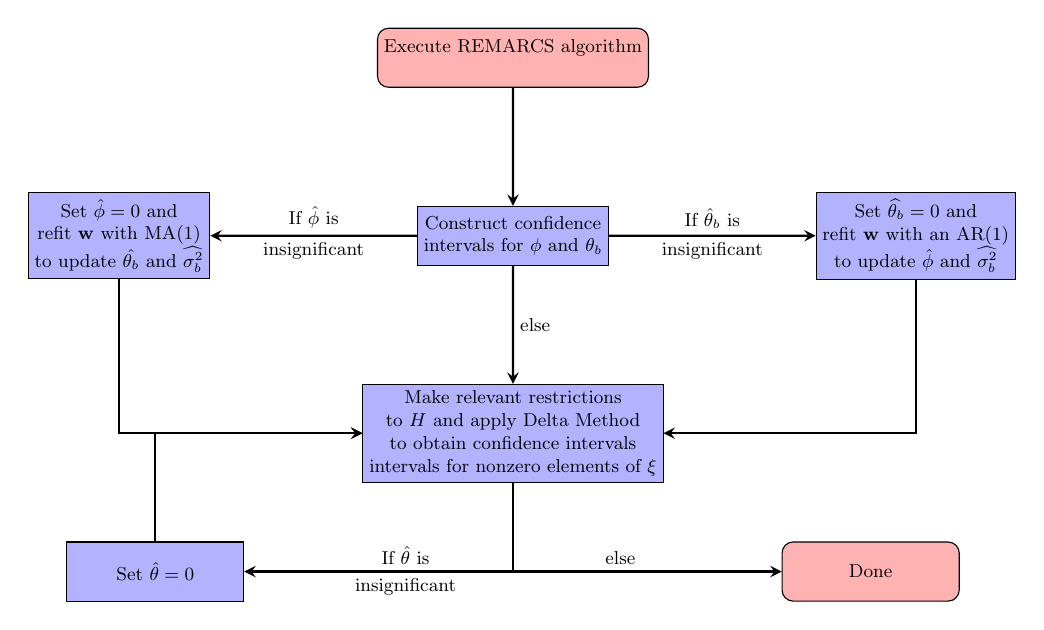
\begin{tikzpicture}[
        scale=.75,
        every node/.style={transform shape},
        node distance=2.5cm
    ]
    \small

    

    \node (start) [startstop, align=center] {
        Execute REMARCS algorithm\\  
    };

    \node (noisehat) [process, below=2cm of start,  align=center] {  
    Construct confidence\\
      intervals  for $\phi$ and $\theta_b$
    };


    \node (observed) [process, below=2cm of noisehat, align=center] {
        Make relevant restrictions\\
        to $H$ and apply Delta Method\\
        to obtain confidence intervals\\
        intervals for nonzero elements of $\xi$ 
    };

    

    \node (phizero) [process,  left=3.5cm of noisehat, align=center] {
        $\text{Set }\hat{\phi}=0$ and\\
        refit $\mathbf{w}$ with MA(1)\\
        to update $\hat{\theta_b}$ and $\widehat{\sigma_b^2}$
    };

    \node (thetabzero) [process, right=3.5cm of noisehat, align=center] {
        $\text{Set }\widehat{\theta_b}=0$ and\\
        refit $\mathbf{w}$ with an AR(1)\\
        to update $\hat{\phi}$ and $\widehat{\sigma_b^2}$
    };

    
    \node (thetainsig) [process, below left=1cm and 2cm of observed] {
        Set $\hat{\theta}=0$
    };


    \node (done) [startstop, below right= 1cm and 2cm of observed] {
        Done\\
        
    };

    % Arrows


    \draw [arrow] (noisehat) -- (observed)
        node[pos=.5, anchor=west]{else};
    
    \draw [arrow] (start) -- (noisehat)
        node[pos=.5, anchor=west]{};

    \draw [arrow] (noisehat) -- (phizero)
        node[pos=.5, anchor=south]{If $\hat{\phi}$ is}
        node[pos=.5, anchor=north]{insignificant};

    \draw [arrow] (noisehat) -- (thetabzero)
        node[pos=.5, anchor=south]{If $\hat{\theta}_b$ is}
        node[pos=.5, anchor=north]{insignificant};

    \draw [arrow] (thetabzero) |- (observed)
        node[pos=.3, anchor=south]{};

    \draw [arrow] (phizero) |- (observed)
    ;
    \draw [arrow] (observed) |- (thetainsig)
        node[pos=.7, anchor=south]{If $\hat{\theta}$ is }
        node[pos=.7, anchor=north]{insignificant }
    ;
    \draw [arrow] (thetainsig) |- (observed)
        
    ;
\draw [arrow] (observed) |- (done)
        node[pos=.7, anchor=south]{else }
        
    ;


    % \draw [arrow] (thetabzerotheta) -- (done);



    % \draw [arrow] (phizerotheta) |- (done);

    \end{tikzpicture}

    \caption{Decision tree for parameter restriction in ARMA--Noise model}
    \label{fig:modelselection}

\end{figure}
\end{center}
\subsection{Generalizing to Varying Sample Size}

Having detailed the steps involved in fitting and performing inference on model 
parameter estimates, we now turn to the condition of constant sample size ($n_t = n$ $\forall$ $ t$),
currently required for fitting an 
ARMA-Noise model. This condition is included so that the time series $\{a_t\}$ is Gaussian 
white noise, and $\mathbf{w}$ is therefore still an ARMA process.

Given that RCS data is rarely of a fixed sample size, we now explore the extent to which this condition can be relaxed whilst $\mathbf{a}$ remains white noise. 
We will now treat $\{n_t\}$ as the realizations of random variables $\{N_t\}_{t=1}^T$. What we aim to establish are the conditions under which the random variable
 $A_t = N_t^{-1}\sum_{i=1}^{N_t}\varepsilon_{ti}$ is still white noise.


\textbf{Claim:}


Let $\{\varepsilon_{ti}\}$ be i.i.d. random variables with
\[
\mathbb{E}(\varepsilon_{ti}) = 0, \qquad \mathrm{Var}(\varepsilon_{ti}) = \sigma_\varepsilon^2 < \infty,
\]
and let $\{N_t\}$ be a stochastic process such that
\[
\Omega(N_t) \subseteq \mathbb{Z}, \quad P(N_t \geq 1) = 1, \quad \mathbb{E}({N_t^{-1}}) = c \quad \text{for all } t,
\]

Define
\[
A_t := \frac{1}{N_t}\sum_{i=1}^{N_t} \varepsilon_{ti}.
\]

Then $\{A_t\}$ is white noise with $\sigma_a^2 = \sigma_\varepsilon^2\,\mathbb{E}(N_t^{-1})$



\textbf{Proof:}

First, let $\{N_t\}$ be i.i.d. random variables with a sample space that is a subset of the integers strictly 
greater than $0$. The conditional random variable $A_t|N_t$ then has variance $\sigma_\varepsilon^2/N_t$. To find the marginal variance Var($A_t$), we use the Law of Total Variation:

\begin{equation}
    \label{eq:totalvar}
    \text{Var}(A_t) = \mathbb{E}(\text{Var}(A_t|N_t)) + \text{Var}(\mathbb{E}(A_t|N_t))
\end{equation}

Now, Var$(A_t|N_t) = \sigma_\varepsilon^2N^{-1}$, and therefore has an expectation of
$\sigma_\varepsilon^2\mathbb{E}(N^{-1})$, which is well defined given that the sample space
of $N_t$ is a subset of the integers strictly greater than zero. At the same time, the expectation of $A$ is $0$
regardless of the value of $N$, meaning the second term in Equation \ref{eq:totalvar} is 
zero, leaving only Var$(A) = \sigma_\varepsilon^2\mathbb{E}(N^{-1})$. 


We can verify that $A_t$ is zero mean with the Law of Total Expectation:
$$ \mathbb{E}(A_t) = \mathbb{E}(\mathbb{E}(A_t|N_t)) = \mathbb{E}(0) = 0 $$

Now we've already established $\text{Var}(A_t)$ to be independent of $t$, so we now 
verify that $\text{Cov}(A_r,A_s) = 0$ for $r \neq s$. The Law of Total Covariance states:


$$ \text{Cov}(A_r,A_s) = \mathbb{E}(\text{Cov}(A_r,A_s|N_r,N_s)) + \text{Cov}(\mathbb{E}(A_r|N_r), \mathbb{E}(A_s|N_s))$$

Given that $A_r$ and $A_s$ are functions of independent random vectors $\bm{\varepsilon}_r \in \mathbb{R}^{n_r}$ and $\bm{\varepsilon}_s \in \mathbb{R}^{n_s}$, $\text{Cov}(A_r,A_s|N_r,N_s)$ must be zero. Having already established that both variables are zero-mean, the above equation reduces to:

$$ \text{Cov}(A_r,A_s) = \mathbb{E}(0) + \text{Cov}(0, 0) = 0$$

\qed

Having shown that $\{A_t\}$ is still white noise, it now remains to estimate its variance. 
Though the sample sizes now vary, our estimate for $\sigma_\varepsilon^2$ hasn't changed (see Equation \ref{eq:var_eps_hat}).
From Argentino (2026) \cite{Argentino2026}, this estimate does assume independence in the
daily sample sizes. If sample sizes display evidence of dependence, then the estimate for
$\sigma_\varepsilon^2$ must be amended to reflect it.




Without requiring the distribution of $N_t$, $\sigma_a^2$ can be estimated with:

\begin{equation}
    \label{eq:var_a_n}
    \hat{\sigma}_a^2 = \frac{\hat{\sigma}_\varepsilon^2}{T}\sum_{t=1}^T\frac{1}{N_t}
\end{equation}

With $\hat{\sigma}_\varepsilon^2$, $\hat{\sigma}_a^2$ and $\hat{\text{Var}}(\hat{\sigma}_\varepsilon^2)$ defined as above, the algorithm proposed by Wong and Miller can be once again applied, with necessary adjustments made to $\Sigma_o$ and $H$. 



% \subsection{ARMA-Noise Models With Stationary Sample Sizes}







The takeaway from all this is that a constant expected inverse of $\{N_t\}$ is the critical piece for $\{A_t\}$ to still be white noise.
Such a condition is satisfied if the sample sizes are the realizations of a \emph{strictly} stationary time series,
but not necessarily if stationarity is weak. The sample sizes don't even have to be of constant mean, 
so long as the expectation of $N_t^{-1}$ is constant \cite{Argentino2026}.

So long as the set of inverse sample sizes $\{n_t^{-1}\}$ is conceivably of constant expectation, the ARMA-Noise method is applicable.

The condition that $P(N_t > 0) = 1$ begs the question of what to do in the event of missing time steps. These instances are 
treated as "missing data", since the method of moments estimator for $\mathbb{E}(N_t^{-1})$ would be undefined if those
instances were included. Only non-zero sample sizes are used to estimate $\mathbb{E}(N_t^{-1})$, and the zeros present 
in the vector of sample sizes will simply correspond to zero-columns in $X_t$ that don't end up affecting 
the outcome, as packages like \textit{arima} can handle missing values.


\subsection{Extending to Mixed Effects Models}

A natural extension of this algorithm is to allow for random effects in addition to fixed ones,
yielding a model of the following form:

\begin{equation}
    \yy = X_f\beta + X_r\mathbf{b} + X_t\uu + \varepsilon, \qquad     \text{Var}(\mathbf{b}) = \Sigma_b
\end{equation}






The algorithm changes only in that the initial model fit includes random effects (\textit{lmer package}) \cite{Bates2015}
The fixed effects estimate $\hat{\beta}_{GLS}$ adjusts in that $\Omega$ now includes the 
term $X_r\Sigma_bX_r'$. Random intercepts $\mathbf{b}$ are updated with the 
conditional expectation $\mathbb{E}(\mathbf{b}|\yy, \hat{\xi}) = \Sigma_b X_r' \Omega^{-1}(\yy - X_f\hat{\beta})$.
Following the EM formulation for variance component estimation
\citep{laird1982variance}, the update for the random-effects
variance is:

\[
\widehat{\sigma}_b^{2\,(k+1)}
=
\frac{1}{m}
\sum_{i=1}^m
\left[
\widehat{b}_i^{\,2}
+
\operatorname{Var}(b_i \mid \mathbf{y})
\right].
\]
A flowchart depicting the steps of the algorithm is given in 
Figure \ref{fig:modelflow}.


\medskip

\begin{figure}[htbp]
    \centering
    \vspace{.5in}
\resizebox{\textwidth}{!}{
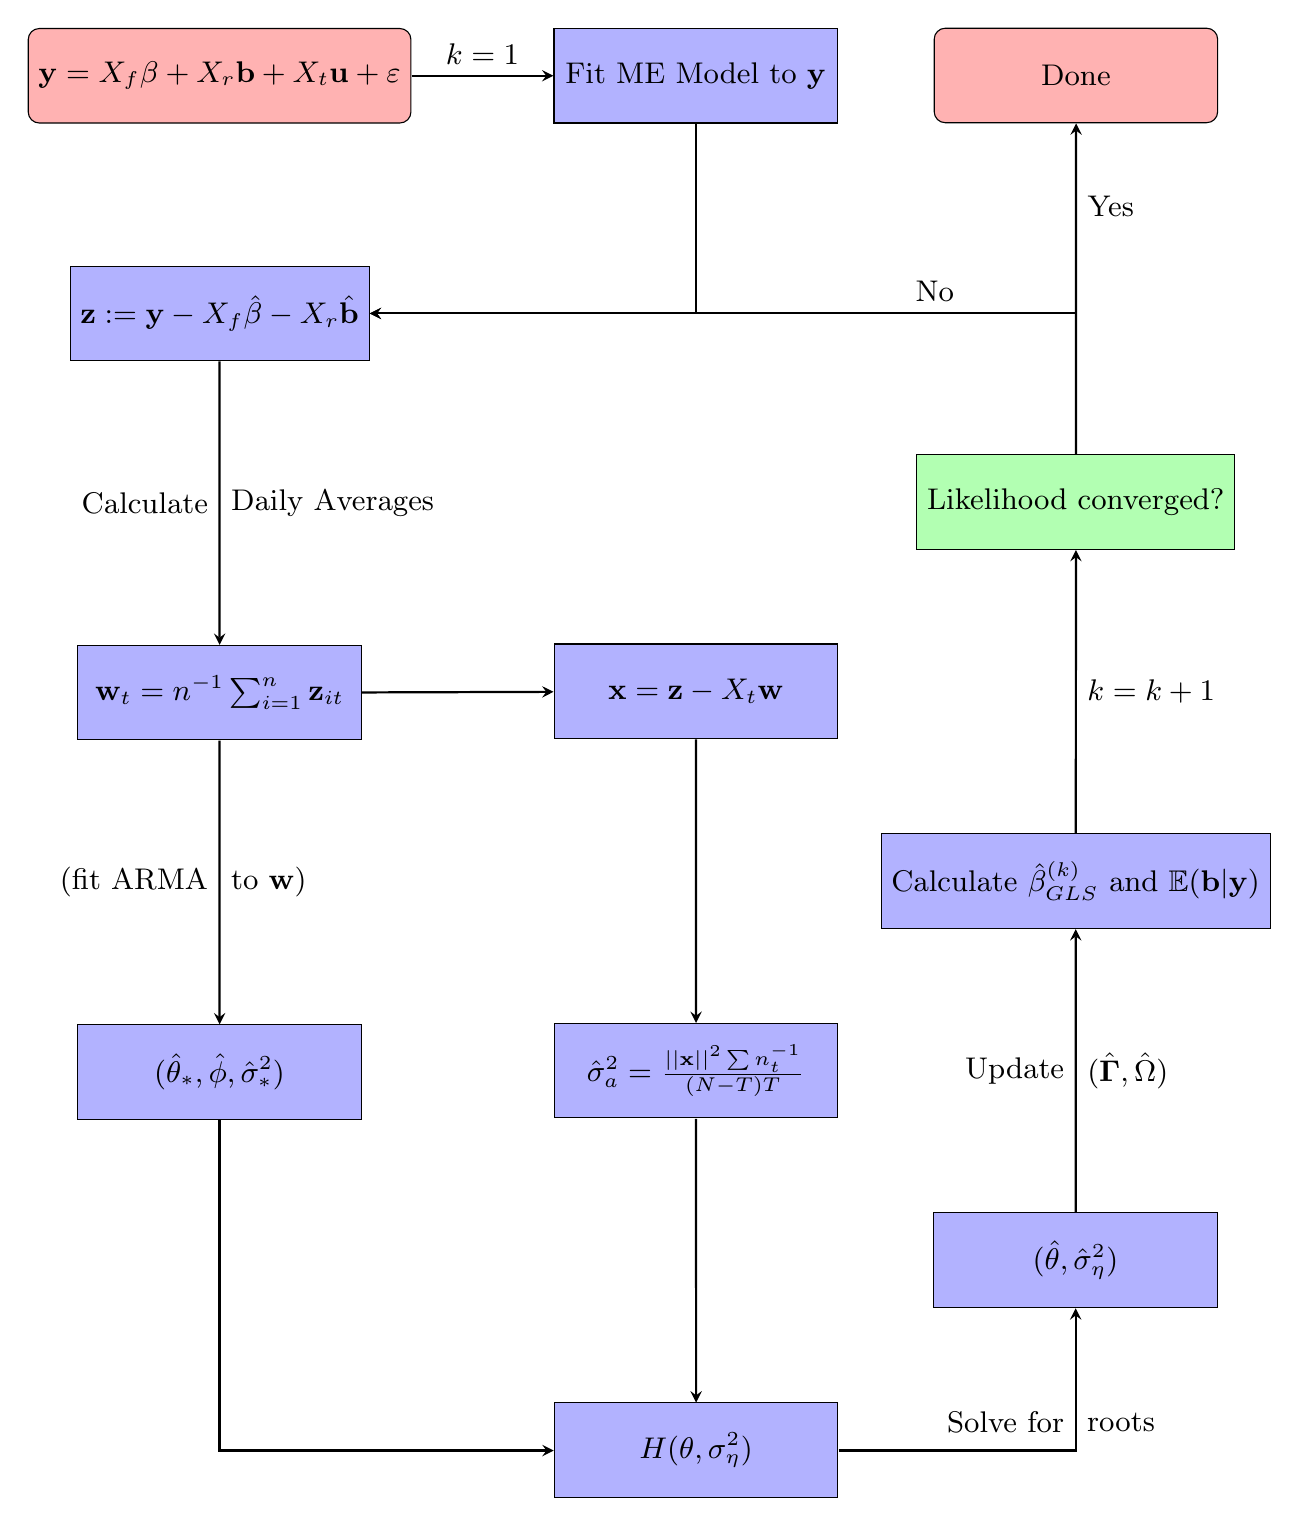
\begin{tikzpicture}[scale=1.2, every node/.style={transform shape}, node distance=2.5cm]{}
\small
    % Nodes vertically aligned
    \node (start) [startstop] {$\mathbf{y} = X_f\beta + X_r\mathbf{b} + X_t\mathbf{u} + \varepsilon$};
    \node (step1) [process, right=1.5cm of start] 
        {Fit ME Model to $\yy$};
    \node (step2) [process, below = 1.5cm of start] 
        {$\mathbf{z}:= \yy - X_f\hat{\beta} - X_r\hat{\mathbf{b}}$};
    \node (step3) [process, below = 3cm of step2] 
        {${\mathbf{w}}_t = n^{-1}\sum_{i=1}^{n} \mathbf{z}_{it}$};
    
    % Parallel branch
    \node (step4a) [process, below = 5.5cm of step1] 
        {${\mathbf{x}} =  \mathbf{z} - X_t\mathbf{w}$};
    \node (step5a) [process, below = 3cm of step4a] 
        {$\hat{\sigma}_a^{2} = \frac{||\mathbf{x}||^2\sum n_t^{-1}}{(N-T)T}$};
    
    \node (step4b) [process, below = 3cm of step3] 
        {$(\hat{\theta}_*, \hat{\phi}, \hat{\sigma}_*^2)$};
    
    \node (step5b) [process, below  = 3cm of step5a] 
        {$H(\theta,\sigma_\eta^2)$};
    
    \node (step7) [process, above right = 1cm and 1cm of step5b] 
        {$(\hat{\theta}, \hat{\sigma}_\eta^2)$};
    
    % % Merge after parallel
    \node (step8) [process, above = 3cm of step7] 
        {Calculate $\hat{\beta}_{GLS}^{(k)}$ and $\mathbb{E}(\mathbf{b}|\mathbf{y})$};
    
    \node (checkll) [decision, above = 3cm of step8] 
        {Likelihood converged?};
    \node (done) [startstop, above = 3.5cm of checkll] {Done};
    
    % Arrows
    \draw [arrow] (start) -- (step1)
        node[pos=0.5, anchor = south]{$k = 1$};
    \draw [arrow] (step1) |- (step2) node[pos=0.5, anchor = south]{};
    \draw [arrow] (step2) -- (step3)
        node[pos=.5,anchor = east]{Calculate}
        node[pos=.5,anchor=west]{Daily Averages};
    \draw [arrow] (step3) -- (step4a) 
        node[pos=.5,anchor = south]{}
        node[pos=.5,anchor=north]{};
    \draw [arrow] (step3) -- (step4b) 
        node[pos=0.5, anchor = east]{(fit ARMA}
        node[pos=.5,anchor=west]{to $\mathbf{w}$)};
    \draw [arrow] (step4a) -- (step5a);
    \draw [arrow] (step5a) -- (step5b);
    \draw [arrow] (step4b) |- (step5b);
    \draw [arrow] (step5b) -| (step7)
        node[pos=.6,anchor = east]{Solve for}
        node[pos=.6,anchor = west]{roots};
    \draw [arrow] (step7) -- (step8)
        node[pos=.5, anchor = east]{Update}
        node[pos=.5, anchor = west]{$(\hat{\GG},\hat{\Omega})$};
    \draw [arrow] (step8) -- (checkll)
        node[pos=0.5, right]{$k = k+1$};
    \draw [arrow] (checkll) -- (done)
        node[pos=.75, anchor = west]{Yes};
    \draw [arrow] (checkll) |- (step2) 
        node[pos=.6, anchor = south]{No};
\end{tikzpicture}
}
    \caption{Flowchart of algorithm steps for estimating model parameters}
    \label{fig:modelflow}
\end{figure}


Derivations excluded for concision can be found in the PhD dissertation on which this work
is based \cite{Argentino2026}. Having described the procedure for parameter estimation and
inference, we now proceed to assess the algorithm's performance. A note on computational speed:
because we aren't relying on pre-compiled functions like \emph{lm}, \emph{arima} and 
\emph{lmer} for updating parameter estimates, we have to calculate estimates manually.
The main computational bottleneck of this procedure is inverting $\Sigma_\yy$. However,
we can expedite this process through the Woodbury equation \cite{woodbury1950}, used once in
the fixed effects setting and twice in the mixed effects setting.


\section{Results}
Before applying this methodology to real data, we first corroborate its necessity and
efficacy through simulations, closely examining individual components of the algorithm
along with pre-existing methods. 

\subsection{Instability of EM Algorithm}

To highlight the necessity for a different approach to fitting latent parameters,
we test the potential stability of time series parameter estimates obtained 
from an EM algorithm that estimates the latent time series $\uu$ through its conditional expectation.
We define our model as follows:

$$ y_{ti} = \mathbf{x}_{ti} \beta + u_t + \varepsilon_{ti}, \qquad t = 1,...,T $$
$$i = 1,...,n_t \qquad n_t \overset{i.i.d.}{\sim} \text{Poi}(\lambda) + 1 $$

Here, $\uu$ is defined to be an AR(1) process with innovation variance $\sigma_\eta^2 = \areveta$. 
Other fixed parameters include $\sigma_\varepsilon^2 = \areveps$, $T = \areT$, and $\beta = c(\areint,\areslope,\arecov)$.
For varying values of $\phi$, $\aresims$ realizations of the model were simulated,
and for each simulation, \emph{true values for all parameters} were used to 
estimate $\hat{\uu} = \Sigma_\uu X_t' \Sigma_\yy^{-1}(\yy - X_f \beta)$. That estimate
was then used to fit an AR(1) model, updating $\hat{\phi}$ just as would be done
via the EM algorithm (in the unlikely event all parameters were unwittingly estimated perfectly).
Results are displayed in Table \ref{tab:are_stability}.

\input{../figures/are_tab.txt}

It is immediately apparent that even in the event of perfect parameter estimation,
conditioning on $\hat{\uu}$ will yield biased estimates for time series parameters if treated as an AR(1) process.
Having demonstrated the need for a different approach to fitting time series parameters, 
we now turn to confirming the effect that additional noise has on ARMA processes..

\subsection{Effect of Noise on ARMA Processes}

We begin by exploring how observation noise impacts parameter estimation for 
AR(1) processes. Take the following model, in which white noise is added to such a process:


\begin{equation}
    w_t = u_t + a_t, \qquad u_t - \phi u_{t-1} = \eta_t    
    \label{eq:ar_bias_model}
\end{equation}

$$ \qquad a_t \overset{i.i.d.}{\sim}N(0,\sigma_a^2), \qquad \eta_t \overset{i.i.d.}{\sim}N(0,\sigma_\eta^2)
$$

For varying values of $\phi$ and fixed parameters ($\sigma_a^2 = \arbiasvara, \sigma_\eta^2 = \arbiasveta, T = \arbiasT$), 
$\arbiassims$ realizations were simulated, each being fit with an AR(1) model and an ARMA(1,1) model.
Figure \ref{fig:ar_bias} displays the aggregate means for both models. It is immediately apparent that
 $\phi$ is only estimated effectively by the latter model, supporting the claim that, 
while $\uu$ may be AR(1), $\mathbf{w}$ is an ARMA(1,1) process. 

\begin{figure}[htbp]
    \centering
    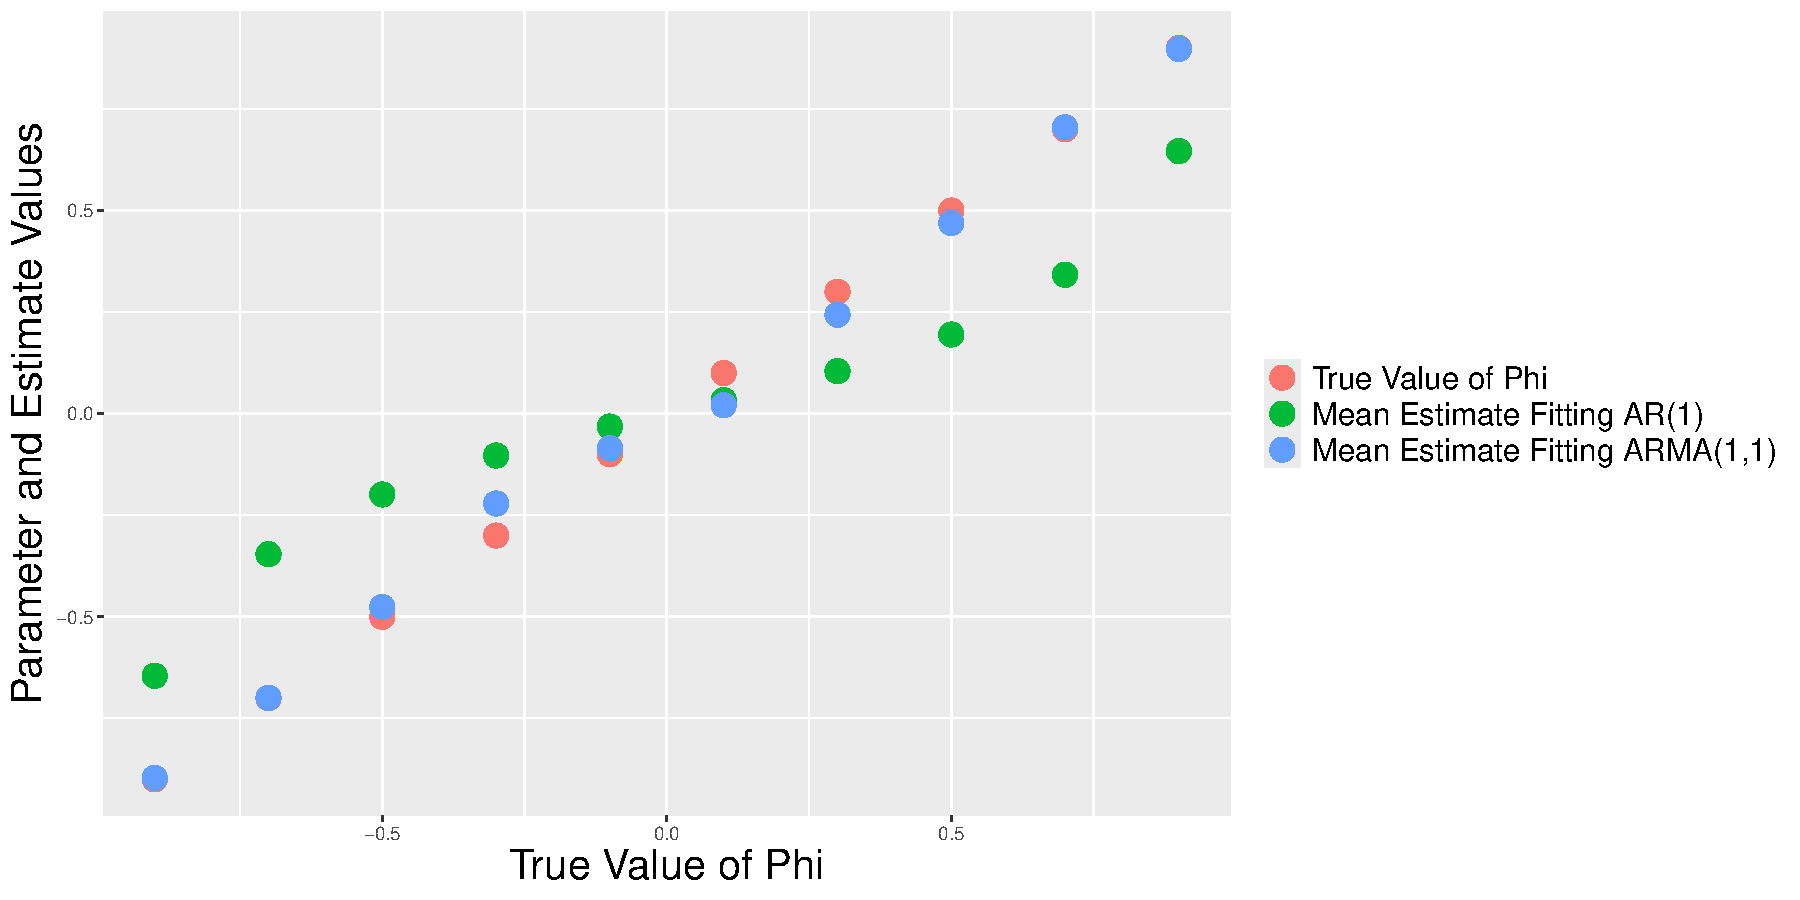
\includegraphics[width=\linewidth]{../figures/ar_bias.pdf}
    \caption[AR bias]{Aggregated estimates for AR parameter of time series with added noise. To see the effect of differing variances, see \href{https://johnargentino.github.io/remarcs_methodological/phi_3d_plot.html}
{this interactive version}}
    \label{fig:ar_bias}
\end{figure}

It is also worth noting that it is not currently possible to tease apart the two sources 
of noise. This is only possible if there are multiple noisy observations of each time series element.
We now proceed to examine the efficacy with which the methodology of fitting ARMA-Noise Models--here generalized for varying sample sizes--does just that.





\subsection{Empirical Confidence of ARMA-Noise Models}
Before applying the REMARCS algorithm in its entirety to simulated data, it would
be prudent to verify that generalizing ARMA-Noise Models to allow for 
varying sample sizes still produces valid estimates.

We begin with simulations of an ARMA(1,1)-Noise Model:
 $$y_{ti} = u_t + {\varepsilon}_{ti}, \qquad u_t - \phi u_{t-1} = \eta_t + \theta \eta_{t-1} $$ 
 
 
 $$\quad t = 1,...,T \quad i = 1,...,n_t \quad n_t \overset{i.i.d.}{\sim} \text{Poi}(\lambda) + 1 $$
 
Differing values of $\phi$ and $\theta$ were combined with fixed parameters $\sigma_\varepsilon^2 = \armanconfveps$, $\sigma_\eta^2 = \armanconfveta$, and $\lambda = \armanconflambda$.
For each value-pair $(\phi,\theta)$, $\armanconfsims$ simulations are generated and used to estimate each combination
parameter values. Confidence regions are then calculated and used to test if true parameter values 
were successfully captured. The empirical confidence levels of varying parameter combinations $(\phi,\theta)$ are depicted
in Figure \ref{fig:e_conf_l}.


\begin{figure}[htbp]
\centering
    \begin{subfigure}{0.55\linewidth}
        \centering
        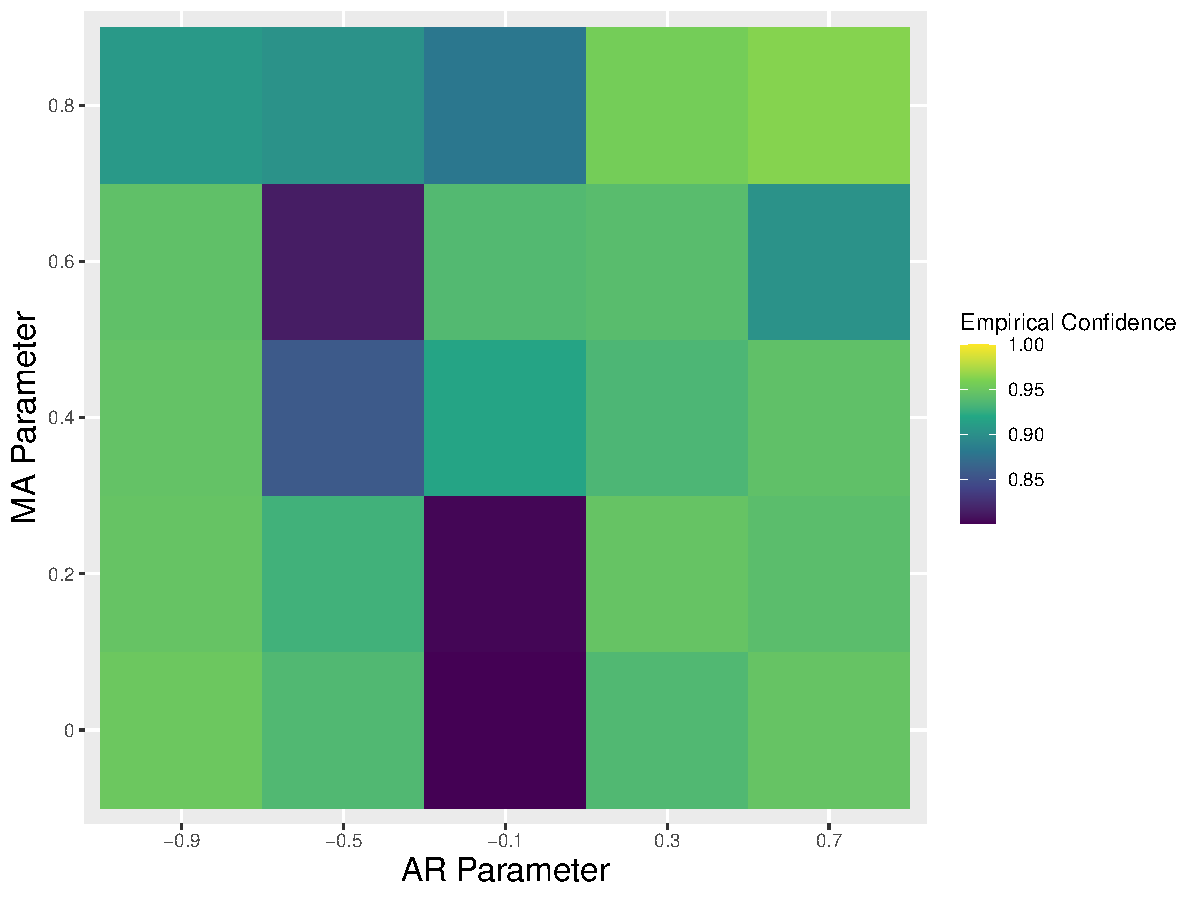
\includegraphics[width=\linewidth]{../figures/e_conf_l_3_2.pdf}
        \subcaption{$T = \armanconfTleft$}
    \end{subfigure}
    \hfill
    \begin{subfigure}{0.41\linewidth}
        \centering
        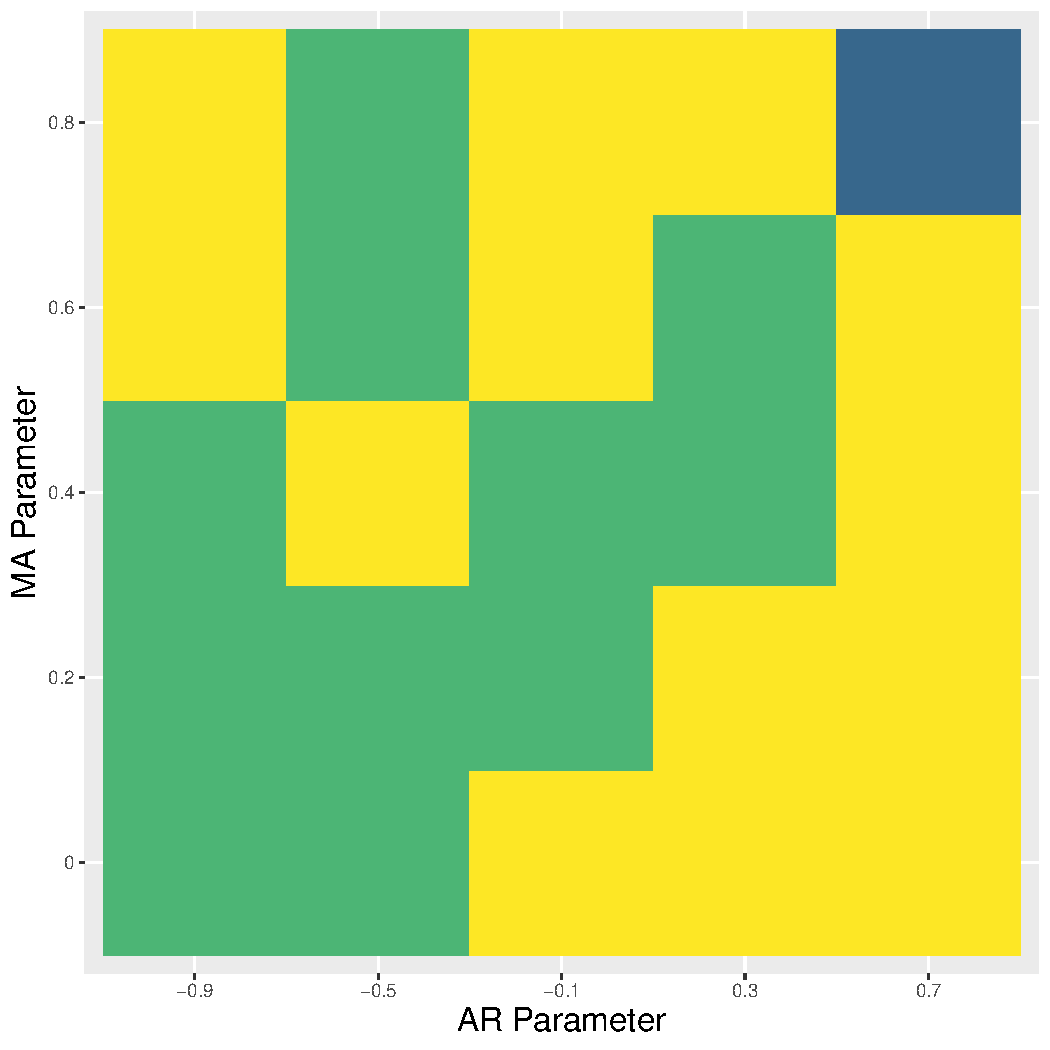
\includegraphics[width=\linewidth]{../figures/e_conf_l_4_2.pdf}
        \subcaption{$T = \armanconfTright$}
        
    \end{subfigure}
    \caption{Rates at which point estimates for $\tau_l$ fall within confidence regions based on sample estimates}
    \label{fig:e_conf_l}
\end{figure}




We can see performance dipped for parameter combinations $(\phi,\theta)$ close to the $\phi + \theta = 0$ line for time series of length $T = \armanconfTleft$. However, we can see that performance improved for $T=\armanconfTright$, suggesting that parameter estimates for ARMA(1,1) processes that resemble white noise take longer to converge to their asymptotic distributions.
Now that we've established that the methodology proposed by Wong and Miller is effective
in estimating parameters governing an ARMA-Noise model, we can add fixed effects to the model.

\subsection{Empirical Confidence of REMARCS algorithm}

Now in order to assess the efficacy of this method, $ \simsfearma $ simulations were conducted with each combination of 
fixed parameters $\beta = (\intfearma,\slopefearma,\xfearma)$, $\sigma_\eta^2 = \vetafearma$, 
$ \sigma_\varepsilon^2 = \vepsfearma$, and varying values of ARMA parameters $(\phi,\theta)$. 

In Figure \ref{fig:conf_heatmap}, we can see the proportion of simulations that yielded 
confidence regions successfully capturing $\beta$ (left) and $(\phi,\theta)$ (right). 
One observation we can make is that, similarly to the ARMA-Noise simulations, convergence
to asymptotic distributions is slower for parameter combinations close to the line $\phi + \theta = 0$. 
This under-performance is mitigated as $T$ grows, indicating that time series more closely resembling white noise 
will require larger values of $T$ for accurate estimation. 


\begin{figure}[htbp]
    \centering
    \begin{subfigure}{0.55\textwidth}
        \centering
        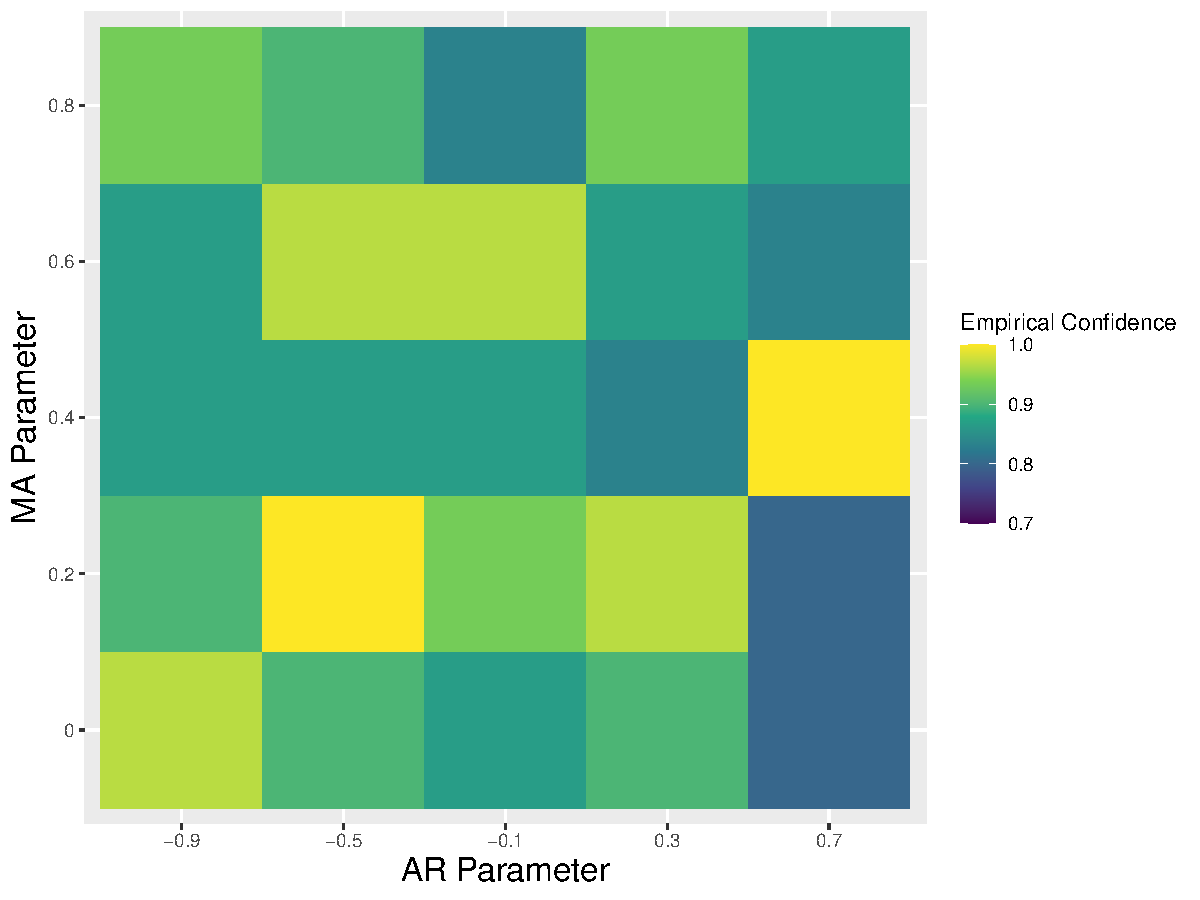
\includegraphics[width=\linewidth]{../figures/l1_conf.pdf}
        \caption{Fixed Effect Parameters \hspace{.5in}}
        \label{fig:sub1}
    \end{subfigure}
    \hfill
    \begin{subfigure}{0.41\textwidth}
        \centering
        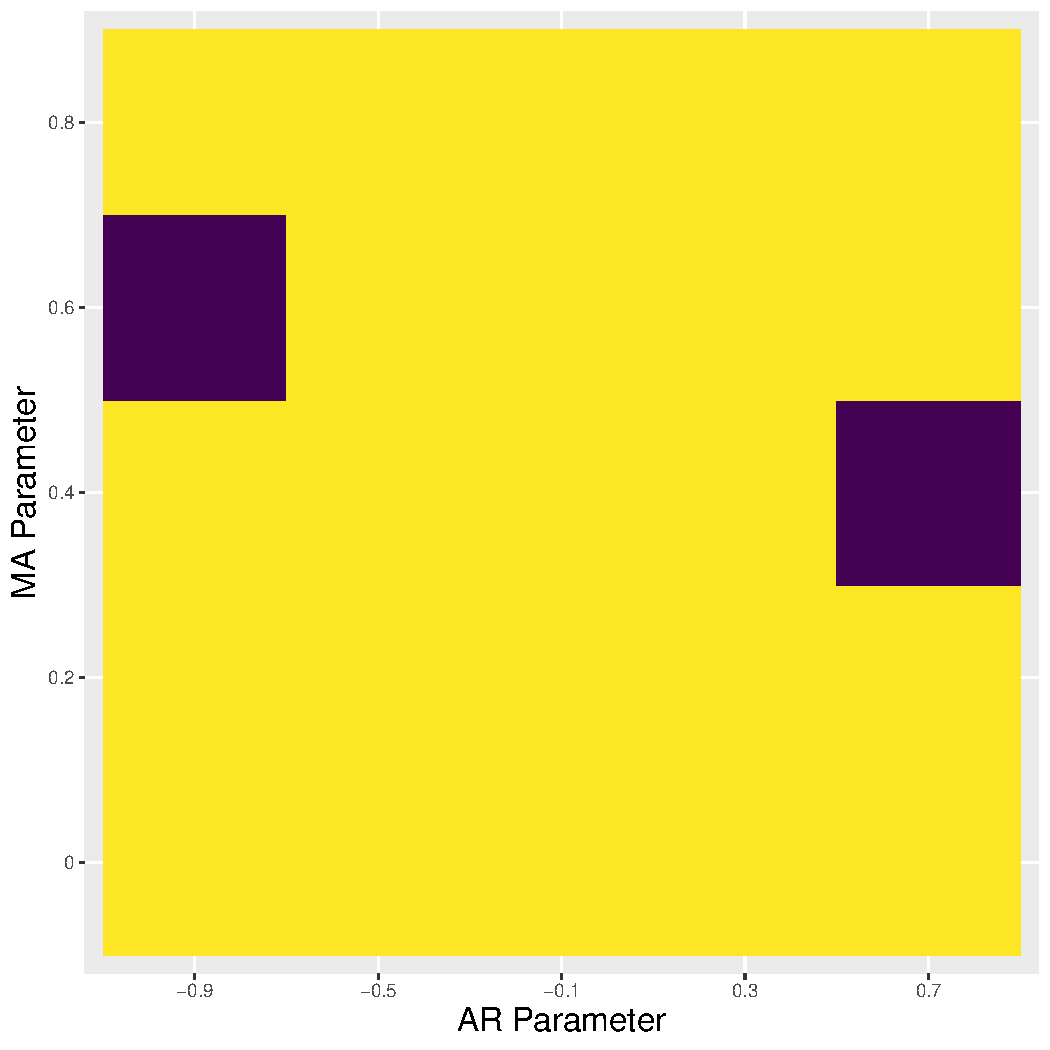
\includegraphics[width=\linewidth]{../figures/l2_conf.pdf}
        \caption{Time Series Parameters}
        \label{fig:sub2}
    \end{subfigure}
    \caption{Empirical confidences with which model parameters fall within confidence regions generated after model convergence}
    \label{fig:conf_heatmap}
\end{figure}
\subsection{Empirical Confidence of Model Selection}


Now that we've seen some aggregate results displaying the efficacy of this method under different parameters,
we aim to evaluate the algorithm's ability to identify when model restriction is necessary.
% \subsection{Case: $\uu$ and $\mathbf{w}$ are ARMA(1,1)}

We start with the case in which $\uu$ is an AR(1) process. We simulate REMARCS models with 
such a latent time series, tracking the rate at which the algorithm yields an insignificant estimate for $\theta$.
Fixed parameters include $T = \uarT$, $\sigma_\eta^2 = \uarveta$, $\sigma_\varepsilon^2 = \uarveps$, $\lambda = \uarlambda$, 
$\beta = (\uarint,\uarslope,\uarcov)$. For each value of $\phi$, $\uarsims$ realizations were simulated
and the REMARCS algorithm applied. Displayed below are the rates at which parameter estimates for 
$\theta$ were deemed insignificant.

\input{../figures/uar_tab.txt}


We now proceed to the case in which $\uu$ is an MA(1) process. We simulate REMARCS models with 
such a latent time series, tracking the rate at which the algorithm yields an insignificant estimate for $\phi$.
Fixed parameters include $T = \uarT$, $\sigma_\eta^2 = \uarveta$, $\sigma_\varepsilon^2 = \uarveps$, $\lambda = \uarlambda$, 
$\beta = (\uarint,\uarslope,\uarcov)$. For each value of $\theta$, $\umasims$ realizations were simulated
and the REMARCS algorithm applied. Displayed below are the rates at which parameter estimates for 
$\phi$ were deemed insignificant.

\input{../figures/uma_tab.txt}

From these results we can see that the algorithm effectively identifies when model restriction is necessary.







\subsection{Method Comparison}

We begin with a realization of a REMARCS model (Figure \ref{fig:sample_are}) with parameters detailed in Table \ref{tab:sample_are}. 
The moving average parameter $\theta$ has been set to zero so the model is consistent with the ARE model detailed by Modugno et al.

Our best attempt to recreate the ARE algorithm encounters convergence problems, likely due to inappropriately
fitting time series estimates with an AR(1) time series.



\begin{table}[htbp]
    \centering
    \begin{tabular}{c|c|c|c|c|c|c|c}
        Parameter   & Intercept     & Slope     &  Dummy Indicator     & $\sigma_\varepsilon^2$    & $\phi$    & $\theta$  & $\sigma_\eta^2$\\
        \hline 
        Value       & $\intrcpt$    & $\slope$      & $\covind$     & $\vareps$                 & $\ar$     & $\ma$     & $\vareta$
    \end{tabular}
    \caption{Parameter values for simulated ARE model}
    \label{tab:sample_are}
\end{table}

\begin{figure}[htbp]
    \centering
    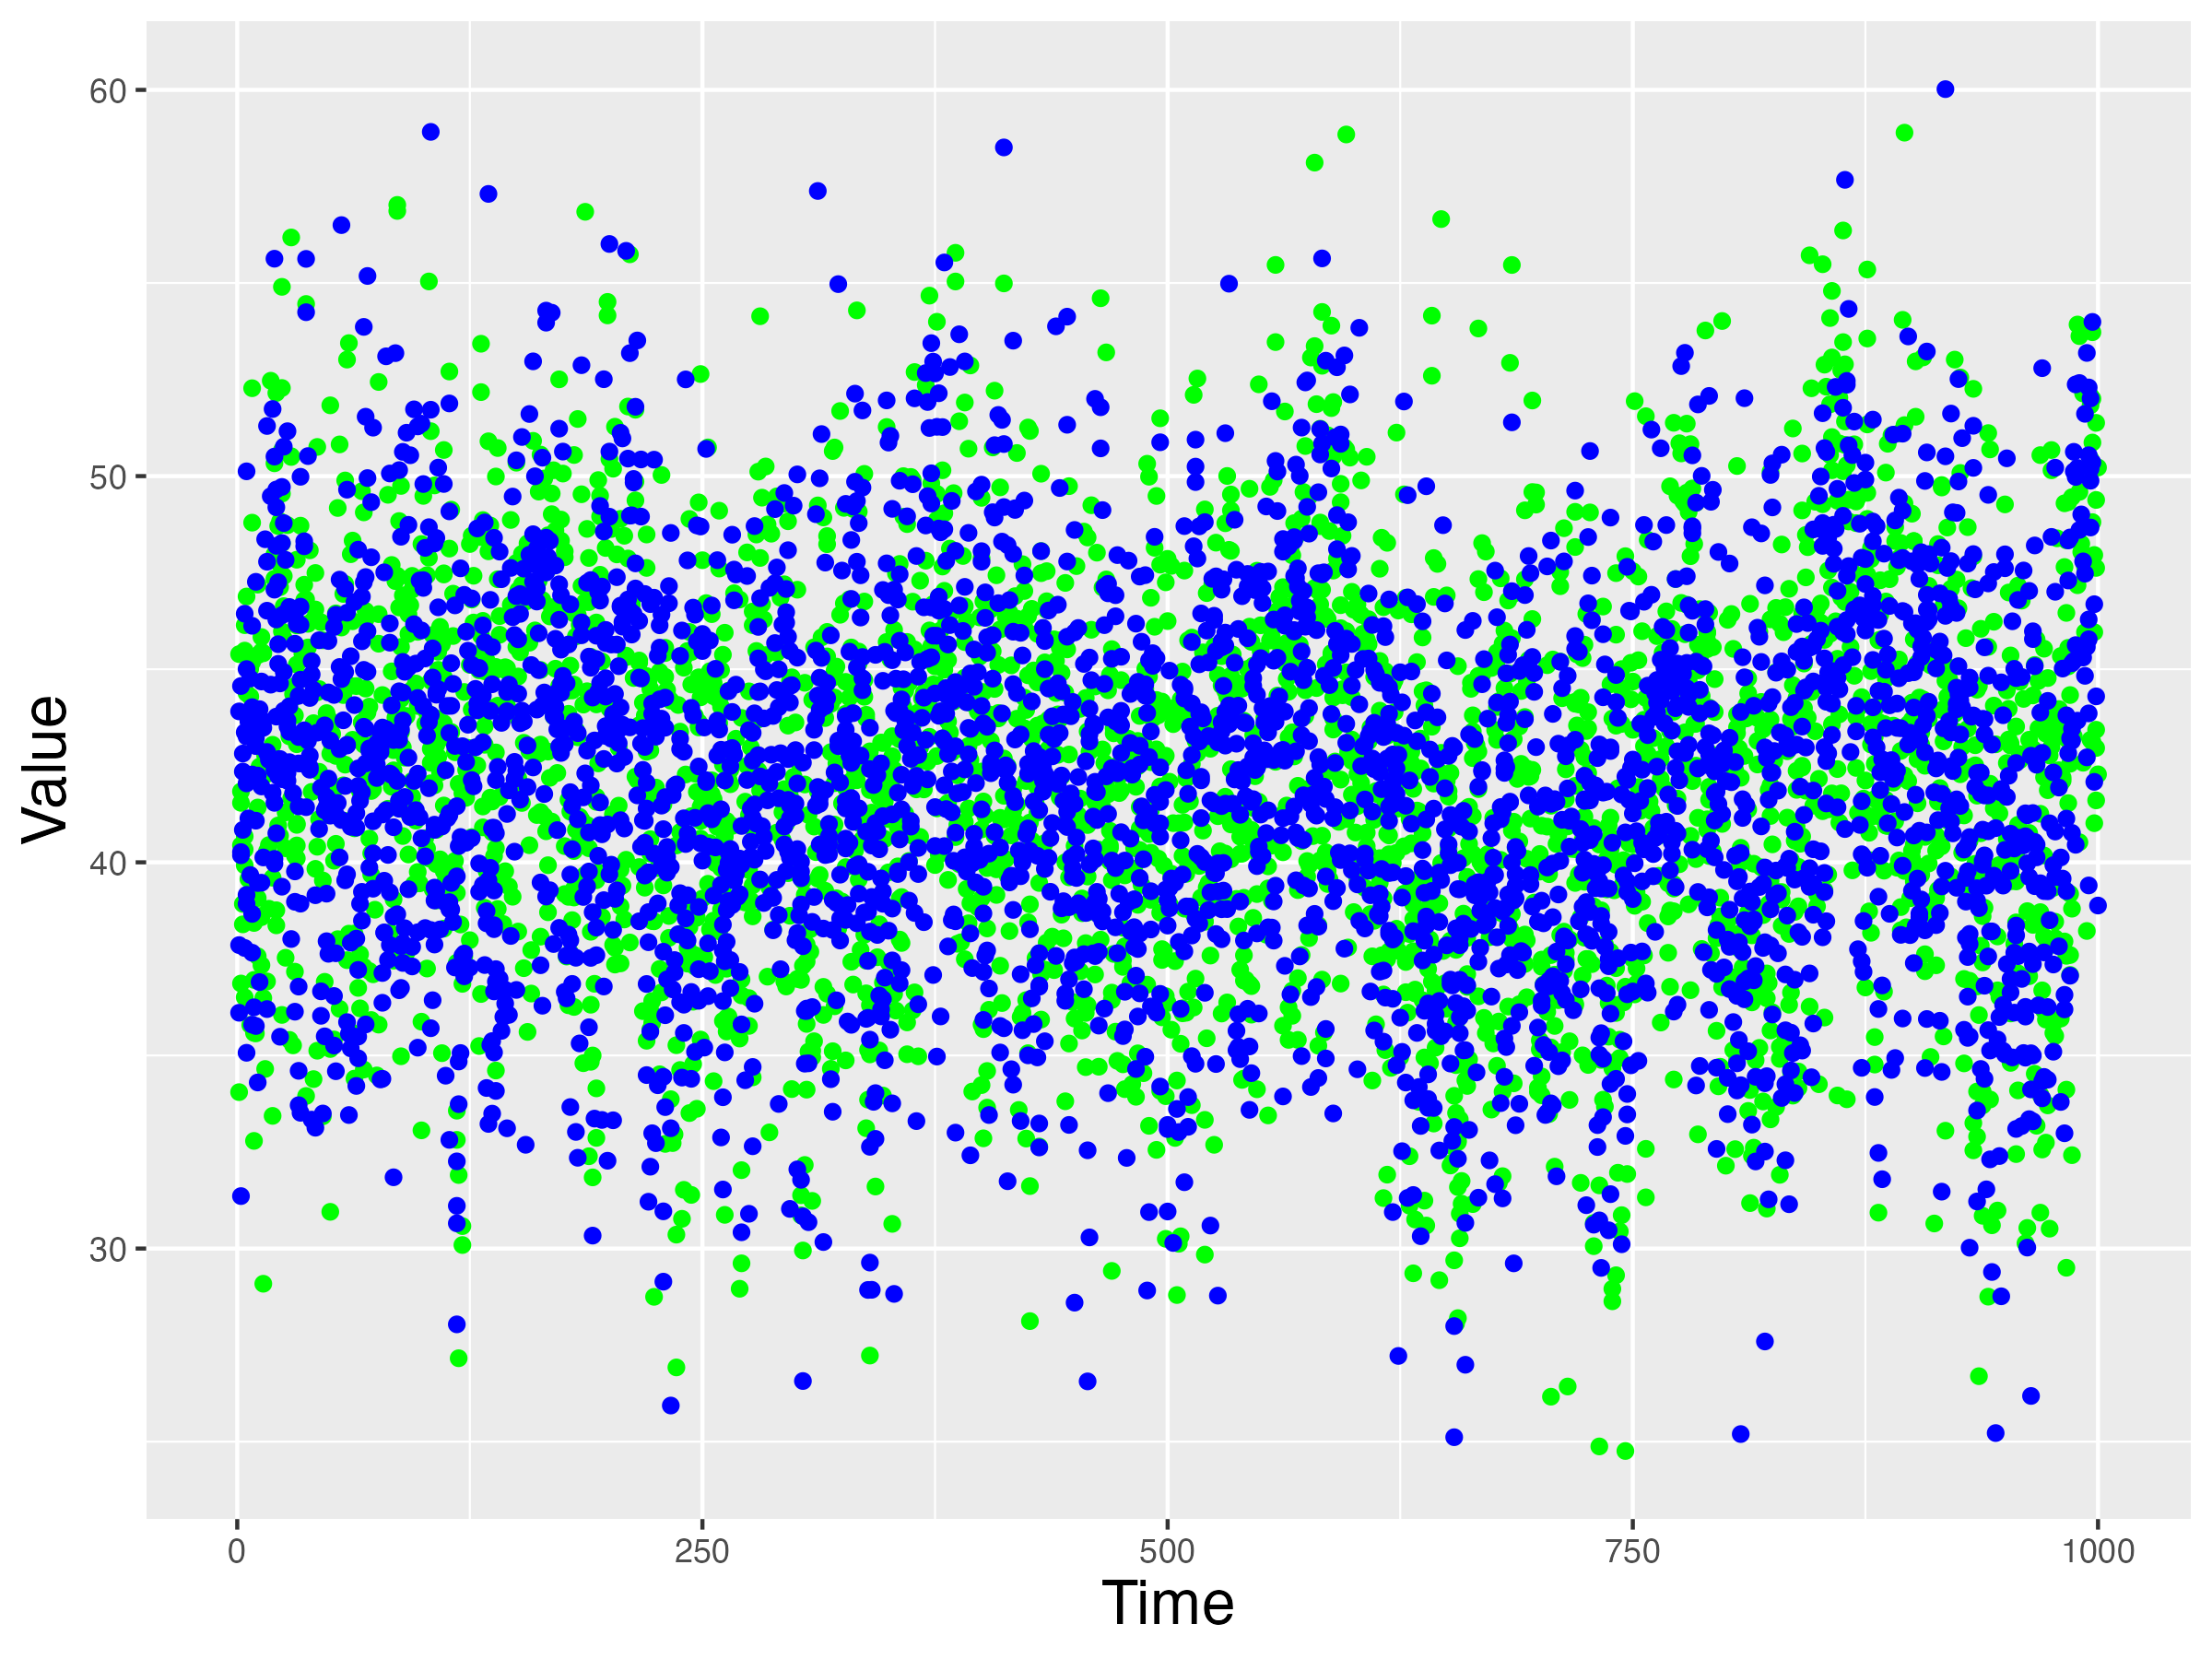
\includegraphics[width=0.6\linewidth]{../figures/are.png}
    \caption{Realization of ARE model with parameters defined in Table \ref{tab:sample_are}}
    \label{fig:sample_are}
\end{figure}

% \subsection{Simulations}

We now compare the performance of the REMARCS algorithm with those of 
the ARE model and fitting a time series with covariates.


We consider fitting this model by aggregating the data at each time point 
and treating the averages as a time series with covariates. $\sims$ 
simulations were generated for each set of parameters and fit with both methods.



Some sample rows of simulated data are provided below:


% \input{../figures/arma_cov_head.txt}

After aggregating at each time step, we obtain the following condensed dataset, from which a time series with 
covariates is then fit:

% \input{../figures/arma_cov_head_daily.txt}

\begin{table}[htbp]
    \centering

    \begin{subtable}[t]{0.48\textwidth}
        \centering
        \input{../figures/arma_cov_head.txt}
        \caption{Individual Data}
        \label{tab:arma_cov_head}
    \end{subtable}
    \hfill
    \begin{subtable}[t]{0.48\textwidth}
        \centering
        \input{../figures/arma_cov_head_daily.txt}
        \caption{Aggregate Data}
        \label{tab:arma_cov_head_daily}
    \end{subtable}

    \caption{Example of the simulated dataset before and after aggregation. Panel (a) shows sample observations from the original simulated data, while panel (b) shows the condensed dataset obtained by aggregating observations at each time step. The aggregated data are subsequently used to fit the time series model with covariates.}
    \label{tab:arma_cov_comparison}
\end{table}

Note that entries of the \textit{x} column, while displaying some variability, are fairly close to $0.5$. 
If we then fit a time series with covariates to the condensed dataset, we obtain results with empirical means 
displayed in the table below. The ``Significance Frequency" column displays the fraction of the $\sims$ 
simulations in which the corresponding parameter estimate was statistically significant at the $\alpha = \tscovalpha$ 
level.


\input{../figures/arma_cov_df.txt}

Note that the effect of the dummy indicator variable is deemed significant only
 $\covconf\%$ of the time (Table \ref{tab:armacov}), whereas the same simulations yield an empirical confidence of $\covconfremarcs\%$ when the REMARCS algorithm is applied (Table \ref{tab:remarcs}). This example highlights the shortcomings of fitting a time series with covariates.
  Also of note is how skewed the sample mean of $\hat{\theta}$ is. This is because what we are in fact estimating is 
  $\theta_b$, the MA parameter of $\mathbf{w}$.


\input{../figures/remarcs_df.txt}










Results displaying the REMARCS algorithm's effect on mobile phone survey data on household food security in Yemen can be found in Argentino et. al., 2025
 \cite{Argentino2026review}. 



\section{Discussion}
% \subsection{Discussion}
This article develops a framework for analyzing high-frequency repeated cross-sectional survey data that exhibit temporal correlation while containing individual-level covariates that are time independent. It does so by introducing a latent ARMA process, inducing an overall ARMA-Noise residual structure, and recursively fitting parameter estimates with GLS and ARMA-Noise methods. In order to accommodate survey data with varying daily sample size, this research furthered ARMA-Noise modeling by relaxing the preexisting condition that sample sizes be constant. Results provide insight into how temporal correlation interacts with cross-sectional noise, particularly how not properly accounting for this interaction can obfuscate results and hinder proper inference. Given how large RCS datasets can be, computational methods were tailored to the specific characteristics of this model by leveraging the relationship between the spectral decompositions of the various covariance matrices involved. The exploration of these models has produced insight into the limitations of their analysis and yielded several interesting directions for further research.
% \section{Interpretation of Key Findings}

A result central to this work is that parameter estimates for a latent ARMA process will be fundamentally flawed if fit to aggregate residuals, as the presence of additional white noise introduces bias in estimates for not only the variance parameter but the moving average parameter as well. Such an impact is tractable, however, and can be reverse engineered to obtain asymptotically unbiased estimates for the true time series parameters. The relation between the observable and latent time series must be incorporated into the analysis of time series estimate. This impact can change the order of the ARMA process on top of the parameters themselves. For instance, in the case that the latent time series is actually an AR(1) process, the observed aggregate errors will be ARMA(1,1) with a moving average parameter of opposite sign as that of the autoregressive parameter. Modeling the noisy time series as an AR(1) process would prevent a consistent estimate for $\phi$ from being obtained. Simulation results reinforce this conclusion. We see that as the relative variance of the additional noise increases, estimates for $\phi$ obtained by fitting an AR(1) model become increasingly biased, while those fit with an ARMA(1,1) model remain accurate.


% \section{Implications}
    This work provides a viable method for analyzing datasets such as the mVAM surveys, elucidating individual-level effects by properly accounting for temporal shocks that would otherwise obfuscate them. Such a method avoids the information loss inherent to the aggregate methods that are currently commonplace.

% \subsection{Methodological}


% \subsection{Practical}
Furthermore, failure to account for temporal correlation when modeling repeated cross-sectional data can lead to invalid inference. At the same time, flattening the data to be analyzed into aggregates results in significant information loss at the individual level. In particular, in the event that individual-level variables like education level or income source see little variance in their prevalence at the time-step level, fitting aggregated data using a time series with covariates could easily obscure an otherwise significant effect.

% \section{Limitations}
    This method is not without limitations, particularly given its reliance on asymptotic distributions. As such confidence regions underperform for low values of T, particularly in boundary cases like $\phi,\theta \approx \pm1$ and $\phi + \theta \approx 0$, as the resulting covariance structure is close to that of white noise. The imposition of an ARMA order no greater than $(1,1)$ is certainly limiting, as it precludes REMARCS Models with all but three types of latent ARMA processes from being properly fit.  

% \section{Directions for Future Research}
    There are a number of natural extensions that arise from this work, particularly 
    generalizing the time series level of the model to allow for $p,q > 1$. Given that 
    survey data so often tracks binary output variables, relaxing the Gaussian condition 
    is of further interest. Since confidence intervals are currently based on asymptotic
    distributions, the derivation of small-sample corrections is warranted. Lastly, 
    while the theory now accommodates samples size that vary, whether it be strictly stationary
    or not in certain circumstances, understanding the effect this has on parameter estimation
    is not yet understood.
% \section{Conclusion}
\section{Data Availability Statement}
The code that produced these results can be found \href{https://github.com/johnargentino/remarcs_methodological}{here}.
% \section{To-Do List}
% \begin{itemize}
%     % \item Sync changes to Fixed and Mixed functions in package
%     \item load package in R Markdown file and alude to it in paper
%     \item Amend code so that likelihood is split based on ybar and not uhat
%     \item Juxtapose bias on uhat and AR plus noise
% \end{itemize}
\bibliographystyle{plain}
\bibliography{../mVAM_refs}
% \section{Appendix}
% \input{sections/appendix.tex}
% \listoftables
% \listoffigures
\end{document}